%%%%%%%%%%%%%%%%%%%%%%%%
% $Autor: RanjeetsingTawar$
% $Pfad: Car_Licence_Plate_Identification_with_a_JetsonNano$
% $Version: 4.0.0 $
%
% !TeX encoding = utf8
%
%%%%%%%%%%%%%%%%%%%%%%%%
\chapter{Data Mining}
For centuries, inventors have aspired to create machines capable of thought, a concept dating back to Ancient Greek civilization. The advent of computers sparked curiosity about whether these machines could ever become self-aware, centuries before the emergence of Artificial Intelligence (AI). AI is an umbrella term covering a variety of technologies, including Machine Learning, Deep Learning, and Artificial Neural Networks. Humans have always been captivated by the idea of building machines that mimic human thought and behavior. The closest achievement to this vision is the development of Artificial Neural Networks, inspired by the decision-making processes of the human brain. Today, numerous advanced technologies, modeled on the principles of the natural world, are capable of tackling highly complex mathematical challenges. The sections that follow explore the mechanisms of some of the most widely used Machine Learning and Deep Learning algorithms.

\section{Machine Learning}
Machine Learning (ML) encompasses algorithms that can autonomously learn and improve through experience without requiring explicit programming for every task. As defined by Mitchell (1997), "A computer program is considered to learn from experience E concerning a class of tasks T and a performance measure P if its performance on tasks in T, evaluated by P, improves with experience E" \cite{Mitchell:1997}. Machine Learning is typically divided into three main categories: Supervised Learning, Unsupervised Learning, and Reinforcement Learning.

\subsection{Supervised Learning}
Supervised learning is the process of finding a function that best approximates the relationship between input data and corresponding outputs based on a given dataset. According to Cord (2008), "Supervised learning entails learning a mapping between a set of input variables X and an output variable Y and applying this mapping to predict the outputs for unseen data" \cite{Cord:2008}. In essence, it refers to algorithms that learn and make predictions independently, given labeled input-output pairs.

Supervised learning is particularly effective for problems involving classification and regression. It involves two main phases:

Training Phase: During this phase, the system is provided with labeled datasets to associate specific inputs with their corresponding outputs. A larger dataset generally leads to better learning outcomes; however, selecting an appropriate dataset is crucial to avoid pitfalls like overfitting (when the model performs well on training data but poorly on unseen data) or underfitting (when the model fails to learn adequately due to insufficient or poor-quality data).

Testing Phase: After training, the system is evaluated using a separate dataset, which lacks labels, to measure its predictive accuracy. This phase ensures that the model can generalize its learning to new, unseen data effectively.

\subsection{Unsupervised Learning}
Unsupervised Learning involves algorithms that analyze and group datasets based on inherent patterns or trends within the data. Unlike supervised learning, unsupervised learning does not rely on labeled data. Instead, the algorithm must identify patterns and relationships on its own. The primary goals of unsupervised learning include uncovering the underlying structure of a dataset, grouping data into categories based on similarities, and compressing the dataset into a more manageable representation.

Unsupervised algorithms are generally categorized into two types: clustering and association.
\begin{enumerate}
	\item Clustering Algorithms: These algorithms group items into clusters based on their similarities. Items within the same cluster share significant commonalities, while those in different clusters have minimal or no similarities. Cluster analysis helps classify data objects based on the presence or absence of shared characteristics \cite{GFG:2024}.
	\item Association Algorithms: These algorithms use association rules to discover relationships between variables within a large dataset. They identify groups of items that frequently occur together in the data.
\end{enumerate}

\subsection{Reinforcement Learning}
Reinforcement learning is a technique that relies on feedback, without the need for labeled datasets. Unlike supervised learning, where the algorithm is provided with labeled data to make decisions, reinforcement learning requires the agent to determine actions to accomplish a task. The correctness of these actions is evaluated through feedback, or reinforcement. In reinforcement learning, decision-making is sequential, meaning each action depends on the previous output, and the outcome of an action is influenced by the current state. Positive reinforcement increases the likelihood of a behavior occurring, while negative reinforcement decreases it. Positive reinforcement is more commonly used in reinforcement learning because it helps models reach their full potential in completing a task.

\subsection{Machine Learning Algorithms}

\subsection{YOLOv5 and CNNs}
YOLOv5 and CNN both extract features from the input image through all the convolutional layers in the detection module. As the number of layers increases, the number of channels grows, while the size of the feature map progressively decreases. \cite{Redmon:2016} The later feature maps contain higher-level features, which are more useful for recognizing the license plate (LP) and predicting its area of interest box.

In this project, TensorFlow versions 2.9.1 and 2.3.1 are used for YOLOv5. Although YOLOv5 is based on PyTorch, it can be cloned from \url{https://github.com/ultralytics/yolo5} by executing the command: ! git clone https://github.com/ultralytics/yolo5, which creates the necessary folder structure for YOLOv5.

The dataset is split into training and validation sets, with 80% used for training and 20% for validation. YOLOv5 first utilizes the Box Regression layer to predict the bounding boxes. Then, EasyOCR extracts the region of interest from the feature maps based on the relative position of the bounding boxes, merges the feature maps after pooling, and feeds the combined maps into the subsequent classifiers.

The YOLOv5 model was trained on the CLPD dataset, and it was customized and fine-tuned according to the dataset’s specific characteristics. During the training pipeline, the input file is processed by cropping the LP from the full image, which is then passed to EasyOCR for text recognition. The file structure and dataset weights are prerequisites for YOLOv5. \cite{Redmon:2016}

The images used for modeling are first converted from BGR to RGB format. These processed images are passed to the detector, which plots bounding boxes around the LP. The region inside these boxes is referred to as the area of interest. After obtaining the results, frames, and classes, the boundary boxes are filtered based on the probability threshold. Only those bounding boxes with a threshold greater than 0.55 are considered for further processing.

\begin{figure}[h!]
	\centering
	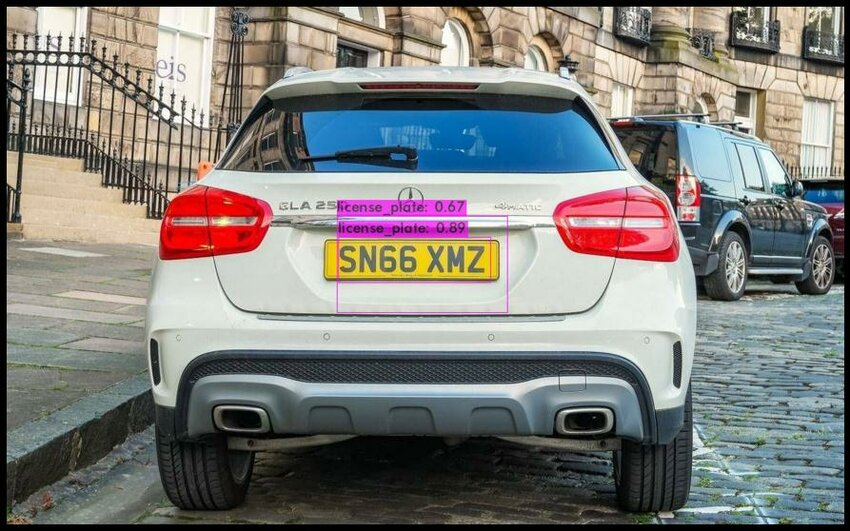
\includegraphics[width=0.7\textwidth]{Images/Two-Bounding-Boxes-Around-the-Number-Plate-There-are-two-bounding-boxes-in-figure-5-with}
	\caption{YOLOv5 Result}
\end{figure}

\subsection{EasyOCR and Keras CNN}
From the boundary box, we can get x and y coordinates, these coordinates are used to recognise the LP using EasyOCR. \cite{Aljelaw:2022}
\begin{figure}[h!]
	\centering
	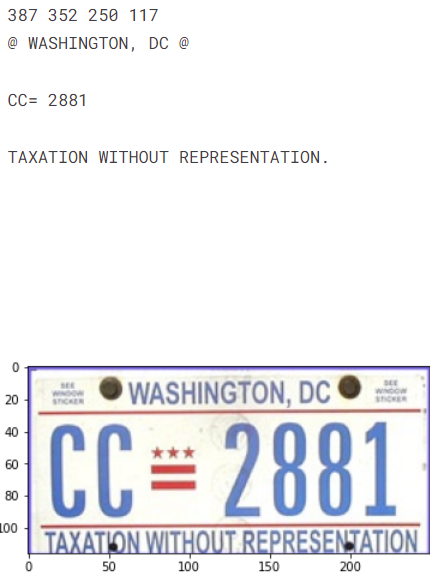
\includegraphics{Images/EasyOCR-result}
	\caption{EasyOCR Result \cite{Aljelawy:2022}}
\end{figure}
\begin{figure}[h!]
	\centering
	
\includegraphics[width=\textwidth]{Images/Tensorflow}
	\caption{Tensorflow Result}
\end{figure}
Keras CNN consists of three convolutional layers with ReLU and Batch Normalization, several MaxPooling layers with Dropout and several components composed of fully connected layers. The last layers has 4 dense layers as it refers to 4 co-ordinates of the LP. \cite{Aljelaw:2022}
\begin{figure}[h!]
	\centering
	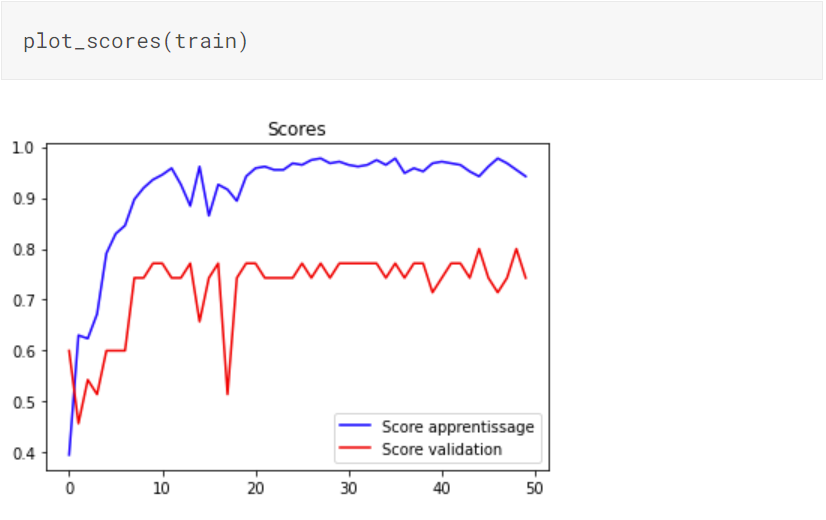
\includegraphics[width=0.8\textwidth]{Images/CNN-Training-Plot}
	\caption{Training and Testing loss}
\end{figure}

\begin{table}[h!]
	\begin{tabular}{m{4cm}|m{4cm}|m{4cm}}
		\hline
		
		Layer (type) & Output Shape & Param \#\\
		
		\hline
		\hline
		
		vgg16 (Functional) & (None, 7, 7, 512) & 14714688\\
		
		\hline
	 	flatten (Flatten) & (None, 25088) & 0\\
	 	dense (Dense) & (None, 128) &  3211392\\
	 	dense\_1 (Dense) & (None, 128) & 16512\\
	 	dense\_2 (Dense) & (None, 64) & 8256\\    
	 	dense\_3 (Dense) & (None, 4) & 260\\ 
	 	\hline
	    \hline
	    \multicolumn{3}{l}{Total params: 17,951,108}\tabularnewline
	    \multicolumn{3}{l}{Trainable params: 3,236,420}\tabularnewline
	    \multicolumn{3}{l}{Non-trainable params: 14,714,688}\tabularnewline
	    \hline
	\end{tabular}
	\caption{\label{tab:Test and Traning data Parameters}Test and Traning data Parameters}
\end{table}


\section{EasyOCR}
%\chapter{Package \PYTHON{Example}}

\index{Example}

\subsection{Description}

ALDPR uses EasyOCR for transforming the raw images of LP. After detecting the area of interest from car images OCR is used in the segmentation of characters. It isolates the character and number from the LP and recognizes the whole sequence of characters.


EasyOCR breakdowns the blobs to locate the character and their bounding box, using one of two segmentation modes:
\begin{enumerate}
	\item Keep object mode: One bob corresponds to one character
	\item Repaste objects mode: The blob is grouped into characters of nominal size. When a blob is big it can be split automatically.
\end{enumerate}

Easy OCR processes the character images to normalize the size into a bounding box, extract relevant feature and stores them in a font file. The patterns in a form are stored as arrays of pixels defined by pattern width and pattern height.

\subsection{Applications of EasyOCR}

\subsection*{Automated Vehicle Monitoring Systems} 

\begin{itemize}
	\item EasyOCR aids in real-time recognition of license plates in busy environments such as highways, parking lots, and toll booths.
	\item Enables seamless vehicle tracking without human intervention.
\end{itemize}
\subsection*{Traffic Law Enforcement}
\begin{itemize}
\item Facilitates automated detection of traffic violations by capturing license plates of vehicles breaking speed limits, running red lights, or engaging in other infractions.
\item Helps in issuing automated tickets and maintaining records for offenders.
\end{itemize}
\subsection*{Parking Management Systems}
\begin{itemize}
\item Integrates with access control systems in gated parking areas to identify vehicles and grant or deny entry based on pre-registered license plates.
\item Reduces manual efforts and improves security in commercial and residential spaces.
\end{itemize}
\subsection*{Toll Collection and Highways}
\begin{itemize}
\item Allows automated toll collection by reading license plates as vehicles pass through toll booths.
\item Minimizes congestion and ensures smooth operation of toll plazas with real-time OCR processing.

\end{itemize}

\subsection{Hyperparameters}
\subsection*{Hyperparameter for EasyOCR Segmentation:} \cite{EasyOCR:2018}
\begin{enumerate}
	\item \textbf{Threshold:} A too-high value thickens black characters on a white background and may cause merging, a too-small value makes parts disappear. 
	\item \textbf{NoiseArea:} Blob areas smaller than this value are discarded. Make sure small character features are preserved.
	\item \textbf{MaxCharWidth,MaxCharHeight:} Maximum character size. If a blob does not fit in a rectangle with these dimensions, it is discarded or split into several parts using vertical cutting lines.
	\item \textbf{CharSpacing:} The width of the smallest gap between adjacent letters. If it is larger than MaxCharWidth it has no effect. If the gap between two characters is wider than this, they are treated as different characters. This stops thin characters being incorrectly grouped together.
	\item \textbf{RemoveBorder:}Blobs near image/ROI edges cannot normally be exploited for character recognition.
\end{enumerate}
\subsection*{Hyperparameters for EasyOCR Recognition:} \cite{EasyOCR:2018}
\begin{enumerate}
	\item \textbf{Load:} reads a pre-recorded font from a disk file.
	\item \textbf{BuildObjects:} The image is segmented into objects or blobs (connected components) which help find the characters. This step can be bypassed if the exact position of the characters is known. If the character isolation process is bypassed, you must specify the known locations of the characters: AddChars and EmptyChars.
	\item \textbf{FindAllChars:} selects the objects considered as characters and sorts them from top to bottom then left to right.
	\item \textbf{ReadText:} performs the matching and filters characters if the marking structure is fixed or a character set filter was provided.
	\item \textbf{Character recognition:} The characters are compared to a set of patterns, called a font.
	\item The best match is stretched to fit in a predefined rectangle and compared to each normalized template in the font database.
	\item A Character set filter can improve recognition reliability and run time by restricting the range of characters to be compared. For instance, if a marking always consists of two uppercase letters followed by five digits, the last of which is always even, it is possible to assign each character a class (maximum 32 classes) then set the character filter to allow the following classes at recognition time: two uppercase, four even or odd digits, one even digit.
\end{enumerate}

\subsection{Input of EasyOCR}

\subsection*{Image Data}
\begin{itemize}
	\item \textbf{Captured still images of vehicles containing license plates.}
	\item \textbf{Format:} PNG, JPEG, or other standard image formats supported by EasyOCR.
	\item \textbf{Examples:} Photos from traffic cameras, parking lot cameras, or manually uploaded images.
\end{itemize}

\subsection*{Video Frames (if video feed is used)}
\begin{itemize}
	\item Individual frames extracted from video streams recorded by the Jetson Nano’s connected camera.
	\item \textbf{Resolution:} Moderate to high (depending on the camera and system requirements).
\end{itemize}

\subsection*{Camera Feed}
\begin{itemize}
	\item Live video feed from a Logitech C270 or similar camera connected to the Jetson Nano.
	\item Input stream resolution should match the EasyOCR capability for text extraction.
\end{itemize}

\subsection*{Preprocessed Image Data}
\begin{itemize}
	\item Cropped regions of interest (ROI) where the license plate is located.
	\item Includes enhancements like noise reduction, resizing, and brightness adjustments to improve recognition accuracy.
\end{itemize}

\subsection{Output of EasyOCR}
\subsection*{Recognized Text}
\begin{itemize}
	\item The alphanumeric characters on the license plate extracted by EasyOCR.
	\item \textbf{Output format:} Plain text or string (e.g., MH12AB1234).
\end{itemize}

\subsection*{Bounding Box Coordinates}
\begin{itemize}
	\item Coordinates of the recognized license plate area in the input image.
	\item \textbf{Format:} List of coordinates (e.g., [x1, y1, x2, y2]).
\end{itemize}

\subsection*{Confidence Score}
\begin{itemize}
	\item A numeric value indicating the accuracy or confidence level of the text recognition.
	\item \textbf{Format:} Decimal (e.g., 0.95).
\end{itemize}

\subsection*{Processed Image with Overlay}
\begin{itemize}
	\item The input image with a bounding box drawn around the detected license plate and the recognized text overlayed.
	\item \textbf{Format:} Modified image saved as PNG/JPEG or displayed in real-time.
\end{itemize}

\subsection*{Logs or Database Entry}
\begin{itemize}
	\item Logs of recognized license plates for future reference.
	\item \textbf{Format:} Stored as CSV, JSON, or in a relational database.
\end{itemize}

\subsection*{Access Control Decision (if integrated)}
\begin{itemize}
	\item Based on the recognized license plate, the system could output an authorization decision (e.g., "Access Granted" or "Access Denied").
	\item \textbf{Format:} Boolean or text response.
\end{itemize}

\subsection*{Alerts or Notifications}
\begin{itemize}
	\item In case of mismatches or unregistered license plates, notifications or alarms can be triggered.
	\item \textbf{Format:} System event or UI display.
\end{itemize}


\subsection{Requirements}
\subsection*{Prerequisite and installation of EasyOCR}

PyTorch is a core dependency for installing the EasyOCR. 

PyTorch 1.9.0 stable version for Windows is installed. A local python interpreter pip package is used. Conda package is used for python virtual interpreter. For GPU enabled system CUDA 10.2 compute platform is used.

After having above configuration following command can be used for installation of PyTorch(1.9.0)

conda install pytorch torchvision torchaudio cudatoolkit-10.2 -c pytorch

After instlling the PyTorch library easyocr is installed with following steps

pip3 install easyocr

\begin{figure}[h!]
	\centering
	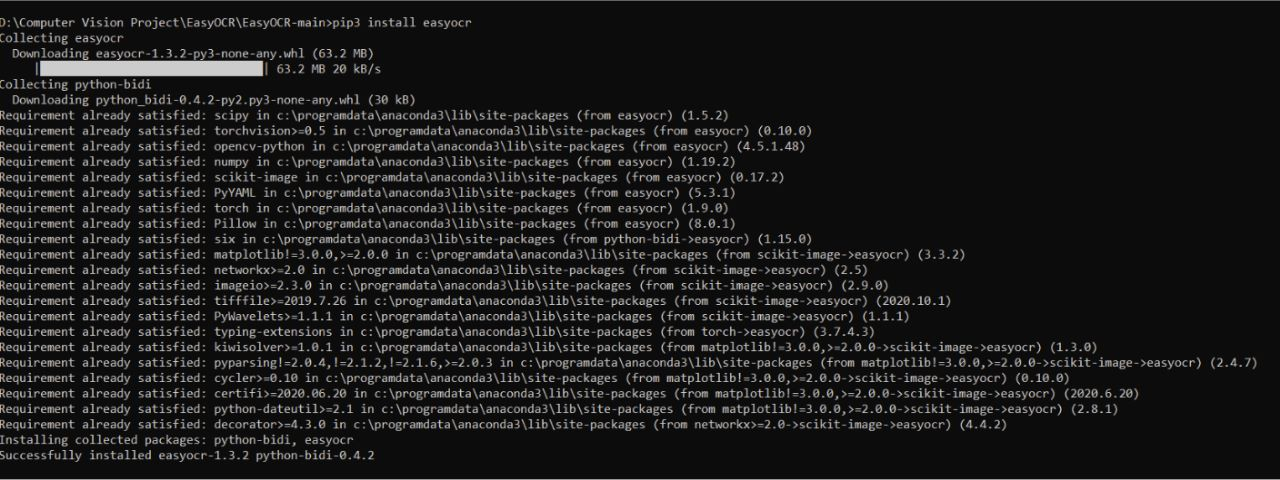
\includegraphics[width=\textwidth]{Images/OCR-Install}
	\caption{EasyOCR Installation using Command Prompt}
\end{figure}

\subsection{Example}
\subsection{Example Manual}
\textbf{Description:} This function facilitates the recognition of license plate numbers using Tesseract OCR. It takes an image, coordinates of the license plate bounding box, an EasyOCR reader object, and a region threshold as input, and returns the recognized license plate number.\newline
\subsection{Example Version}
\textbf{Version:} EasyOCR supports Python 3.6 and above.\newline
Python Version Support for EasyOCR

\subsection*{Officially Supported Versions}
Unfortunately, the project's development appears to be inactive, with the last release occurring in January 2021. The official documentation doesn't explicitly specify supported Python versions.

\subsection*{Community Insights}
Community reports and usage suggest functionality primarily with Python 3.6 and 3.7. Using other versions, particularly Python 2.7 (which reached end-of-life in 2020), is highly discouraged due to potential compatibility issues and security vulnerabilities.

\subsection*{General Recommendations}
\begin{itemize}[label=--]
	\item For the best experience and compatibility, it's strongly recommended to use Python 3.7.
	\item If you must use older Python versions, proceed with caution, thoroughly test your implementation, and be aware of potential limitations or conflicts.
	\item Explore alternative, actively maintained OCR libraries if compatibility with newer Python versions or regular updates are essential. Some well-regarded options include:
	\begin{itemize}[label=$\bullet$]
		\item pytesseract
		\item Textract
		\item pyzbar
	\end{itemize}
\end{itemize}

\subsection*{Additional Considerations}
Be aware that EasyOCR relies on external dependencies, each with their own Python version support details. Check the documentation for each dependency to ensure compatibility with your chosen Python version.

Remember, while EasyOCR might work to some extent with different Python versions, using officially supported and actively maintained libraries generally ensures reliability, security, and access to bug fixes and improvements.

\subsection{Example Files}
\textbf{recognize\_plate\_easyocr.py:} Python script containing the function to recognize license plate numbers using Tesseract OCR.
\subsection{Sample Code ALDPR}
Sample code for EasyOCR:
\begin{lstlisting}
	# function to recognize license plate numbers using Tesseract OCR
	def recognize_plate_easyocr(img, coords,reader,region_threshold):
	# separate coordinates from box
	xmin, ymin, xmax, ymax = coords
	# get the subimage that makes up the bounded region
	# take an additional 5 pixels on each side
	# nplate = img[int(ymin)-5:int(ymax)+5, int(xmin)-5:int(xmax)+5]
	nplate = img[int(ymin):int(ymax), int(xmin):int(xmax)] 
	# cropping the number plate from the whole image
	ocr_result = reader.readtext(nplate)
	text = filter_text(region=nplate, ocr_result=ocr_result,
	region_threshold= region_threshold)
	if len(text) ==1:
	text = text[0].upper()
	return text
\end{lstlisting}
\subsection{Example Description}
The provided function recognize plate easyocr is designed to extract and recognize license plate numbers from images using Tesseract OCR. It first separates the coordinates from the bounding box, then extracts the subimage representing the license plate region. The function then applies Tesseract OCR to the extracted region, obtaining an OCR result. Finally, the recognized text is filtered using a specified region threshold, and if a single candidate is identified, it is returned as the recognized license plate number. This function serves as a fundamental tool for automating license plate recognition tasks in various applications, including vehicle monitoring and traffic management systems.\newline
\subsection{Example EasyOCR}
In the above code snippet, we just need to focus on few points:
\begin{enumerate}
	\item Instead of detecting one-line text, here we are looping through all the detection as we want to plot multiple lines of text.
	\item While giving the coordinates on cv2.putText we are using an extra variable which is “spacer” this spacer later in the code is being incremented to +15 which is helping to restrict the text to collide over each other.
	\item This spacer variable will help the text to remain sorted and equally spaced
\end{enumerate}
\begin{lstlisting}
	img = cv2.imread(IMAGE_PATH)
	spacer = 100
	for detection in result:
	top_left = tuple(detection[0][0])
	bottom_right = tuple(detection[0][2])
	text = detection[1]
	cv2.rectangle(img, top_left, bottom_right, (0, 255, 0), 3)
	cv2.putText(img, text, (20, spacer), cv2.FONT_HERSHEY_SIMPLEX, 0.5, (0, 255, 0), 2, cv2.LINE_AA)
	spacer += 15
	plt.imshow(img)
	plt.show()
\end{lstlisting}
\subsection{Further Reading}
Challenging and Invalid recognition settings:
\begin{enumerate}
	\item MaxCharWidth, MaxCharHeight: if a blob does not fit within a rectangle with these dimensions, it is not considered a possible character (too large) and is discarded. Furthermore, if several blobs fit in a rectangle with these dimensions, they are grouped, forming a single character. The outer rectangle size should be chosen such that it can contain the largest character from the font, enlarged by a small safety margin.
	\item MinCharWidth, MinCharHeight: if a blob or a group of blobs does fit in a rectangle with these dimensions, it is not considered a possible character (too small) and is discarded. The inner rectangle size should be chosen such that it is contained in the smallest character from the font, shrunk by a small safety margin.
	\item RemoveNarrowOrFlat: Small characters are discarded if they are narrow or flat. By default, they are discarded when they are both narrow and flat.
	\item CharSpacing: if two blobs are separated by a vertical gap wider than this value, they are considered to belong to different characters. This feature is useful to avoid the grouping of thin characters that would fit in the outer rectangle. Its value should be set to the width of the smallest gap between adjacent letters. If it is set to a large value (larger than MaxCharWidth), it has no effect.
	\item CutLargeChars: when a blob or grouping of blobs is larger than MaxCharWidth, it is discarded. When enabled, the blob is split into as many parts as necessary to fit and the amount of white space to be inserted between the split blobs is set by RelativeSpacing. This is an attempt to separate touching characters.
	\item RelativeSpacing: when the CutLargeChars mode is enabled, setting this value allows specifying the amount of white space that should be inserted between the split parts of the blobs.
\end{enumerate}
\subsection{Advanced Tuning}

These recognition parameters can be tuned to optimize recognition:
\begin{itemize}
	\item CompareAspectRation: when this setting is on, EasyOCR is less tolerant of size and takes into account the measured aspect ratio. Using this mode improves the recognition when characters look similar after size normalization as it enforces the difference between narrow and wide characters.
	\item Filtering the characters can be used if the marking structure is fixed.
	\item When objects are larger than the MaxCharWidth property, they can be split into as many parts as needed, using vertical cutting lines.
	\item ESegmentationMode, character isolation mode defines how characters are isolated:
	Keep objects mode: a character is a blob 
\end{itemize}


\section{YOLO V5}
%\chapter{Package \PYTHON{Example}}

\index{Example}

\subsection{Description}
YOLOv5 is a family of compound-scaled object detection models trained on the COCO dataset, and includes simple functionality for Test Time Augmentation (TTA), model ensembling, hyperparameter evolution, and export to ONNX, CoreML and TFLite.

Yolov5 and CNN use extracted features from the input image by all the convolutional layers in the detection module. As the number of layers increases, the number of channels increases and the size of the feature map decreases progressively. \cite{Redmon:2016}
The later feature map has higher-level features extracted and thus is more beneficial for recognizing the LP and predicting its area of interest box.


\subsection{Hyperparameter}
Hyperparameter for YOLOv5: \cite{EasyOCR:2018}
\begin{enumerate}
	
	\item \textbf{Learning-rate start (lr0): }At each iteration, the learning rate begins to determine the step size. For example, if you set the learning rate (0.1) before training, your training progress will rise by 0.1 at each repetition.
	\item \textbf{Learning-rate end (lr1): }learning rate end, which is used to test the following condition,
	\item \textbf{Momentum: }Momentum is the gradient descent algorithm's tuning parameter; its job is to replace the gradient with an aggregation of gradients.
	\item \textbf{Mosaic: }Mosaic is used to improve model accuracy by combining many photos to generate a single image, which is then utilized for training. It is well-known for data augmentation and the discovery of optimum feature approaches.
	\item \textbf{Degree: }Degree is used to improve model accuracy by randomly rotating pictures in the training data up to 360 degrees. This option is especially useful for detecting objects in numerous positions/angles. 
	\item \textbf{Scaling: }Scaling is used to shrink a picture to fit the grid size or to optimize the results. 
	\item \textbf{flipud: }flipud is used to randomly flip photos up and down from the whole dataset in order to achieve better results. This may be taken into account in the data augmentation approach. 
	\item \textbf{fliplr: }fliplr is used to randomly flip photos left and right from the whole dataset in order to achieve better results. This may be taken into account in the data augmentation approach.
	\item \textbf{Weight-decay: }A regularization approach that works by adding a penalty term to a network's cost function, causing the weights to shrink/compress throughout the backpropagation process. 
	There are several more parameters, such as warmup epochs, warmup momentum, and so on, whose values may be modified according on the use case.
\end{enumerate}

\subsection{Installation}
Prerequisite and installation of YOLOv5:

PyTorch is a core dependency for installing the YOLOv5. 

PyTorch 1.9.0 stable version for Windows is installed. A local python interpreter pip package is used. Conda package is used for python virtual interpreter. For GPU enabled system CUDA 10.2 compute platform is used.

After having above configuration following command can be used for installation of PyTorch(1.9.0)

conda install pytorch torchvision torchaudio cudatoolkit-10.2 -c pytorch

After instlling the PyTorch library YOLOv5 is installed with following steps:

YOLO V5 is cloned from \url{https://github.com/ultralytics/yolo5} by running the command

\begin{lstlisting}
	! git clone https://github.com/ultralytics/yolo5. 
	##This will create the folder structure for YOLO V5.##
\end{lstlisting}

Following is the folder sturcture for YOLOv5:
Folder Structure of YOLOv5
/input/data/prepro/
/images/*.png
/train
/validation
/lable/*.xml
/Dataset/
/train/images
/train/images

% Input:
\subsection{Input}
\begin{enumerate}
	\item \textbf{Image or Video Frame:}
	\begin{itemize}
		\item YOLO v5 takes an image or a video frame as input for object detection.
		\item In the context of image detection, the algorithm processes a single image at a time. For video detection, each frame of the video is processed independently.
	\end{itemize}
	\item \textbf{Preprocessing:}
	\begin{itemize}
		\item Before feeding the input image to YOLO v5, preprocessing steps may be applied. Common preprocessing includes resizing the image to a specific input size, normalizing pixel values, and handling color channels.
	\end{itemize}
	\item \textbf{Tensor Representation:}
	\begin{itemize}
		\item The input image is converted into a tensor, which is a multi-dimensional array. This tensor is then used as the input to the neural network.
	\end{itemize}
\end{enumerate}

% Output:
\subsection{Output}
\begin{enumerate}
	\item \textbf{Bounding Boxes:}
	\begin{itemize}
		\item YOLO v5 predicts bounding boxes around objects present in the input image.
		\item Each bounding box is represented by four coordinates (\(x, y\)) for the top-left corner and (\(width, height\)) of the box.
	\end{itemize}
	\item \textbf{Class Probabilities:}
	\begin{itemize}
		\item For each detected bounding box, YOLO v5 assigns class probabilities to indicate the likelihood of the object belonging to a particular class.
		\item These probabilities are often represented as confidence scores, indicating how certain the model is about the presence of a specific object class.
	\end{itemize}
	\item \textbf{Class Labels:}
	\begin{itemize}
		\item YOLO v5 assigns class labels to the detected objects based on the highest class probability.
		\item The class labels correspond to the categories that the model has been trained to recognize (e.g., "person," "car," "dog").
	\end{itemize}
	\item \textbf{Output Format:}
	\begin{itemize}
		\item The output is usually in the form of a list or an array containing information about all detected objects in the image or video frame.
		\item Each element in the list corresponds to a detected object and includes the bounding box coordinates, class probabilities, and class label.
	\end{itemize}
	\item \textbf{Post-processing:}
	\begin{itemize}
		\item After obtaining the raw output, post-processing steps are often applied to filter and refine the results.
		\item Non-maximum suppression is a common technique used to remove redundant bounding boxes and keep only the most confident predictions.
	\end{itemize}
	\item \textbf{Visual Representation:}
	\begin{itemize}
		\item Optionally, the output can be visually represented by drawing bounding boxes around detected objects on the input image or video frame.
		\item This step is essential for interpreting and understanding the results, especially in applications where a visual output is required.
	\end{itemize}
\end{enumerate}


\subsection{Example}
\subsection{Example Manual}
\textbf{Description:} This manual provides instructions for training a YOLOv5 model for license plate recognition using a custom dataset. It covers cloning the YOLOv5 repository, installing dependencies, downloading and preparing the dataset, and initiating the training process.\newline
\subsection{Example Version}
\textbf{Version:} YOLOv5 supports Python 3.8 and above.\newline
Python Version Support for YOLOv5

\subsection*{Officially Supported Versions}
\begin{itemize}[label=--]
	\item \textbf{Python 3.7 and above:} This is the minimum supported version. You can use the yolov5 package from PyPI for easy installation and integration.
	\item \textbf{Python 3.8 (Recommended):} While 3.7 is acceptable, YOLOv5 recommends using Python 3.8 for better performance and compatibility with dependencies.
\end{itemize}

\subsection*{Additional Notes}
\begin{itemize}[label=--]
	\item While older versions like Python 3.6 might work with custom installations and manual dependency management, it's not officially supported and can lead to compatibility issues.
	\item For specific functionalities like training, different requirements might apply. Refer to the official YOLOv5 documentation for detailed information about each feature and its compatibility matrix.
\end{itemize}

\subsection*{Helpful Resources}
\begin{itemize}[label=--]
	\item YOLOv5 GitHub repository: \url{https://github.com/ultralytics/yolov5}
	\item YOLOv5 PyPI package: \url{https://pypi.org/project/yolov5/}
	\item YOLOv5 documentation: \url{https://docs.ultralytics.com/}
\end{itemize}

\subsection{Example Files}
\textbf{train\_license\_plate.py:} Python script containing the code for training the YOLOv5 model.
\subsection{Sample training for YOLOv5}
Sample code for YOLOv5:
\begin{lstlisting}
	# Save this code in a file, for example, train_license_plate.py
	import os
	# Clone YOLOv5 repository
	if not os.path.exists("yolov5"):
	os.system("git clone https://github.com/ultralytics/yolov5")
	# Change directory to yolov5
	os.chdir("yolov5")
	# Install dependencies
	os.system("pip install -U -r requirements.txt")
	# Download sample dataset 
	os.system("wget https://github.com/your_username/your_dataset.zip")
	os.system("unzip your_dataset.zip -d data")
	# Train YOLOv5
	!python train.py --img 416 --batch 16 --epochs 300 --data data/alpr.yaml
\end{lstlisting}
\subsection{Example Description}
This code snippet automates the process of training a YOLOv5 model for license plate recognition. It first checks if the YOLOv5 repository exists; if not, it clones the repository from the official GitHub page. Next, it navigates to the cloned repository directory and installs the necessary dependencies using pip. Then, it downloads a sample dataset from a specified URL and unzips it into the 'data' directory within the YOLOv5 repository. Finally, it initiates the training process with the specified parameters, including image size, batch size, number of epochs, and the path to the dataset configuration file.

This example demonstrates how to set up and execute the training process for a YOLOv5 model tailored for license plate recognition, facilitating the development of custom object detection solutions.\newline


Dataset is divided into training and validation datasets. 80\% of the data for training and 20\% data for validation.
YOLOv5 first exploits the Box Regression layer to predict the bounding box. Then, referring to the relative position of the bounding box in each feature map, EasyOcr extracts the region of interest from several already rendered feature maps, merge them after pooling and feeds the combined features maps to the subsequent Classifiers.

Images that are used for modelling are first converted from BGR to RGB. These processed images are passed to the detector. The detector will plot the boxes around the LP. The region of boxes will be called the area of interest. These functions After getting results, frames and classes, filter out the boundary boxes based on the probability threshold. All the boundary boxes which have a threshold greater than 0.55 are considered for further processing.

From Section 5.1.4:
\begin{figure}[h!]
	\centering
	\includegraphics[width=0.7\textwidth]{Images/YOlOv5}
	\caption{YOLOv5 Result}
\end{figure}
%\nocite{Abadi:2016}

% Überschrift ein Level unter `refsection=chapter`, also \subsection*:
%\printbibliography[heading=subbibliography, segment=\therefsegment]
\subsection{Further Reading}
YOLOv5 encompasses a wealth of resources spanning research papers, official documentation, tutorials, video content, online courses, community forums, conference presentations, and books. The YOLOv5 research paper, authored by Alexey Bochkovskiy, Chien-Yao Wang, and Hong-Yuan Mark Liao, serves as a foundational text, delving into the architecture, methodology, and performance evaluation of YOLOv5. Complementing this, the official GitHub repository of YOLOv5 hosts the source code, documentation, and community discussions, offering a comprehensive resource for understanding and implementing the model.
Practical insights and implementation guidance can be gleaned from tutorials and blog posts available on platforms like Medium and Towards Data Science, while video tutorials on YouTube provide visual walkthroughs of YOLOv5 implementation with PyTorch. Formal education is also available through online courses such as the Deep Learning Specialization on Coursera and the Computer Vision Nanodegree on Udacity, which cover object detection techniques, including YOLOv5. Engaging with community forums like r/computervision on Reddit and Stack Overflow facilitates interaction with peers and experts, fostering knowledge exchange and problem-solving. Additionally, staying updated with conference presentations and workshops, such as those held at CVPR, offers insights into the latest advancements and applications of YOLOv5. For in-depth exploration, books like "Deep Learning for Computer Vision" by Rajalingappaa Shanmugamani provide comprehensive coverage of object detection methodologies, potentially including detailed discussions on YOLOv5. Through these diverse avenues of learning, enthusiasts and practitioners alike can gain a thorough understanding of YOLOv5, from its theoretical underpinnings to practical implementation techniques.

\section{Convolutional Neural Networks}

Complex tasks such as pattern and object recognition with high-dimensional data sets lead to convergence problems and high computation times with conventional approaches. Such tasks can be solved with deep learning algorithms. To this class belong CNN. They can solve tasks with less preprocessing than is usual for other classification algorithms. Moreover, the filters used do not have to be designed by the user, but are learned by the network itself during training. \cite{Saha:2018}

According to \cite{Sharma:2018}, one of the first successful implementations of CNNs was the recognition of handwritten digits in 1998, which is described in the paper \glqq Gradient-Based Learning Applied to Document Recognition\grqq \cite{LeCun:1998}. In the meantime, CNNs have been able to prove themselves in many application areas. The typical application for CNNs is processing data that has a known network topology. For example, they can recognise objects in images or patterns in time series. \cite{Namatevs:2017} Besides image classification, object recognition and tracking, text, speech and gesture recognition are also typical applications \cite{Gu:2018} describes. But CNNs are also used in industry for defect detection. \cite{LopezdeLacalle:2020}

In general, cnn are composed of the building blocks Convolutional Layer, Pooling Layer and Fully Connected Layer, where each building block is usually used more than once. These building blocks are described below. The primary assumption is the use of cnn for image classification.

\subsection{Convolutional Layer}

The main component of CNN are filters that are applied to the input data/images in the Convolutional Layer. As input, the Convolutional Layer receives an n-dimensional tensor, for example an image with three colour channels, and applies several kernels to it. By convolution of tensor and kernel, the image is filtered. The results of the convolution with the different filters are stacked so that the result is again a tensor. \cite{Michelucci:2019}

The operation of convolution between two matrices or tensors means the addition of the products of the multiplication of the corresponding elements of both matrices or tensors. Since the convolution in the Convolutional Layer usually takes place between a tensor with many entries and a small kernel, the convolution must be carried out separately for individual parts of the input tensor. Usually, one starts with the first entries at the top left and, metaphorically speaking, shifts the kernel after the first convolution relative to the input tensor by a certain number of columns and calculates the convolution again. When one has reached the right edge, the kernel is shifted in the row and the process is repeated. The value called stride indicates by how many columns and rows the kernel is shifted relative to the input tensor. In addition, an activation function is usually applied for each calculated pixel. \cite{Michelucci:2019}

In this process, a tensor with dimensions $h_1 \times w_1 \times d_1$ and kernels each with dimension $h_2 \times w_2 \times d_1$, which are stacked to form dimensions $h_2 \times w_2 \times d_2$, becomes an output tensor with dimensions $h_3 \times w_3 \times d_2$. \cite{Arunava:2018}

Here $h_3$ and $w_3$ depend on the height and width of the input tensor as well as the filters and the chosen stride, while $d_2$ is given by the number of filters.

If the size of the input tensor, the kernel and the stride do not match accordingly, pixels at the edge of the image cannot be reached according to the procedure described above. Therefore, sometimes additional pixels are added. This is called padding, or zero-padding, because the added pixels are usually filled with the value zero. \cite{Michelucci:2019}

The parameters learned in a CNN are the filters themselves. For $k$ filters of dimension $m \times n$, considering one biasterm per filter, a total of $k \cdot m \cdot n + k$ parameters must be learned. It is worth noting that this number is independent of the size of the input image, whereas in conventional feed-forward networks the number of weights depends on the size of the input.\cite{Michelucci:2019}

The convolutional layer does not necessarily have to be the first layer, but can also receive preprocessed data as input. Usually, multiple Convolutional Layers are used.\cite{Michelucci:2019}

The filters of the first Convolutional Layer detect low-level features such as colours, edges and curves, while higher layers detect more abstract features. By stacking multiple Convolutional and Pooling Layers, higher level feature representations can be progressively extracted. Moreover, the dimensionality is also reduced continuously, which reduces the computational cost. \cite{Gu:2018,Saha:2018}


\subsection{Pooling Layer}

Usually, each Convolutional Layer is followed by a Pooling Layer. Sometimes both are referred to together as one layer because no weights are learned in the pooling layer. \cite{Michelucci:2019}

It reduces the resolution of the previous feature maps by compressing them, thus reducing complexity and hence computational cost. It also makes the network more robust to small variations in the learned features and focuses on the most important patterns. \cite{Namatevs:2017}


There are different types of pooling. The most common are maximum and average pooling. In maximum pooling, only the maximum value is stored from each section of the tensor covered by the kernel. With average pooling, on the other hand, the average value is determined for each section. \cite{Saha:2018}

The pooling layer does not introduce any new learnable parameters, but it does introduce two new hyperparameters, namely the dimension of the kernel and the stride. \cite{Michelucci:2019}

\subsection{Fully Connected Layer}

After several convolutional and pooling layers, the image is flattened into a single vector. This output is fed into a neural feed-forward network (one neuron per entry in the vector). This is fully interconnected and thus able to extract the non-linear correlations from the extracted features and thus arrive at a classification.\cite{Saha:2018}

The ReLu function is usually used as the activation function. In the output layer, the softmax function is used to reflect the probabilities of each class to be assigned. \cite{Arunava:2018}


\subsection{Hyperparameter}

When building and/or training a CNN , several parameters need to be considered. The architecture of the network and the order of the layers need to be determined. There are new approaches to different convolutional methods from which to choose. In addition, the size and number of filters and the stride must be defined. The pooling procedure must also be defined, as well as the activation functions in the fully networked layers. Likewise, it must be defined how many neurons the input layer should have (this influences the possible image size) and how many layers and neurons per layer the Fully Connected Layer should be composed of.

Many considerations must be made regarding the database. The complexity of the network to be trained depends mainly on whether only one input channel (black and white or greyscale) is used or three (RGB). If only one colour channel is to be used to reduce complexity, the images must be prepared accordingly. Likewise, the size (number of pixels, height and width) of the images may need to be adjusted to fit the architecture used. Normalising the images can also be helpful.

Since the images are presented to the neural network as data arrays, the file format does not play a direct role. Indirectly, however, the different image qualities of the various formats can influence the performance of the networks. For example, networks trained with high-resolution images may produce poor results when they are asked to classify compressed images. \cite{Dodge:2016} Differences can also arise from the different compressions, so different file formats should not be mixed.

\subsection{Fine-tuning}

Fine-tuning allows specific layers from the convolution layer to be trained specifically. With a small number of training images, the mesh can be easily transferred to a new task. This is much faster than designing a neural network from scratch. \cite{Chollet:2018}		

\subsection{Feature Extraction}

In feature extraction, convolutional layers (convolutional layer and pooling layer) are extracted from a trained CNN and a new classifier, i.e. a fully connected layer with new classifications, is added. Two problems arise in this process:

\begin{itemize}
	\item The representation only contains information about the probability of occurrence of the class trained in the basic model.
	\item The fully connected layer contains no information about where the object is located.
\end{itemize}

Should the position of an object in the image matter, the fully connected layers are largely useless, as the later layers only generate abstract concepts. \cite{Chollet:2018}

\subsection{AlexNet}
The most popular CNNs for object detection and classification from image data are AlexNet, GoogleNet and ResNet50. \cite{Sharma:2018}

Gu et al. \cite{Gu:2018} refer to the development of AlexNet in 2012 as a breakthrough in large-scale image classification. Nevertheless, its architecture is only comlpex enough to keep its operation comprehensible. Therefore, it seems a good choice for first attempts at your own training.


AlexNet consists of five Convolutional Layers and three Fully Connected Layers. The number and size of the filters as well as their stride are shown in table \ref{ConvAlex} for the sake of clarity. The first and second convolutional layers are each followed by a response normalisation layer, also known as batch normalisation. This additional layer is intended to mitigate the effect of unstable gradients through normalisation. After the response normalisation layers as well as after the fifth convolutional layer, a max-pooling layer follows. Overlapping pooling was chosen as the pooling method. This means that the individual sections to which pooling is applied overlap. The pooling area measures 3x3 and the stride 2 pixels. ReLu is applied to the output of each Convolutional Layer and each of the Fully Connected Layers. Each Fully Connected Layer consists of 4096 neurons. The output layer uses the softmax function to map the probabilities for the different categories via the output neurons. \cite{Krizhevsky:2012,Alake:2020}



\begin{table} [H]
	\centering
	\begin{tabular} {l l l l l}
		Convolutional Layer & Anzahl Kernel & Dimension & Stride \\ \hline
		1 & 96 & $11\times11\times3$ & 4\\
		2 & 256 & $5\times5\times48$ & 1\\
		3 & 384 & $3\times3\times256$ & 1\\
		4 & 384 & $3\times3\times192$ & 1\\
		5 & 256 & $3\times3\times192$ & 1\\
	\end{tabular}
	\caption{Convolutional Layer Specifications}
	\label{ConvAlex}
\end{table}

In total, AlexNet consists of 650000 neurons. About 60 million parameters need to be trained. \cite{Krizhevsky:2012}

This puts it about in the middle compared to the number of learnable parameters in other successful CNNs.


The input images for AlexNet need to be cropped to size $227 \times 227$. Three colour channels are used (see table \ref{ConvAlex}), so no conversion to greyscale is necessary, but one usually normalises the data to mean 0 and standard deviation 1.\cite{Alake:2020}



\subsection{Image Classification with CNN}


The classification of images is divided into two areas: image classification and object classification. 
Object classification attempts to identify one or more objects. The identification is done by assigning them to predefined classes. As a rule, the results are given with probabilities. Image classification attempts to identify a suitable description for the image; in this case, the image is recorded and interpreted in its entirety. \cite{Zhiqiang:2017}

Several challenges exist when classifying images. If one uses images, one is processing larger amount of data. An image with $200 \times 200$ pixels has 40,000 pixels. If it is a colour image with three colour channels, one processes 120,000 attributes. 
Furthermore, it is desirable that the result of the classification is independent of affine mappings. That is, the result is independent of scaling or rotation of the image. If only a section of the image is examined, the corresponding result should still be delivered. The mapping represents an image with corresponding operations.  
The classic \glqq Lena\grqq{} of image processing is used as the basis of the demonstration \cite{Munson:1996}. This is an image of Lena Soderberg from 1972 that is available in the USC-SIPI Image Database \cite{Weber:1997}.



\begin{figure}[!h]
	\centering
	\begin{tabular}{cc}
		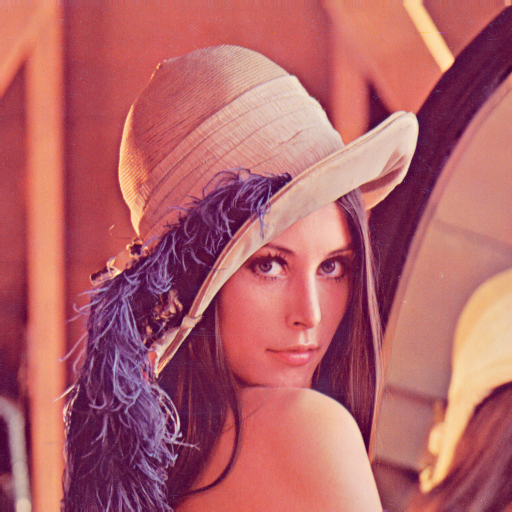
\includegraphics[width=0.4\textwidth]{Images/lena}    &
		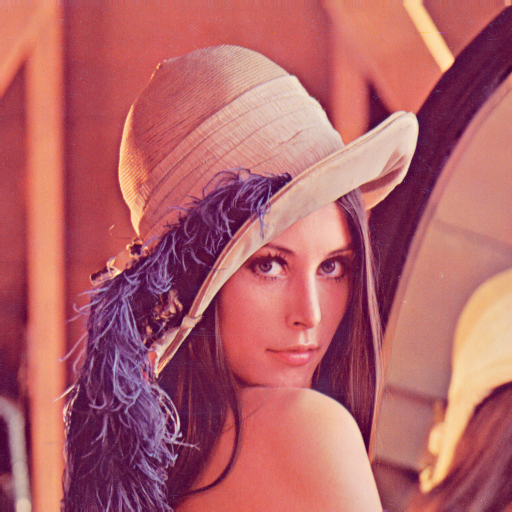
\includegraphics[width=0.4\textwidth,trim=30 30 90 90,clip]{Images/lena}    \\
		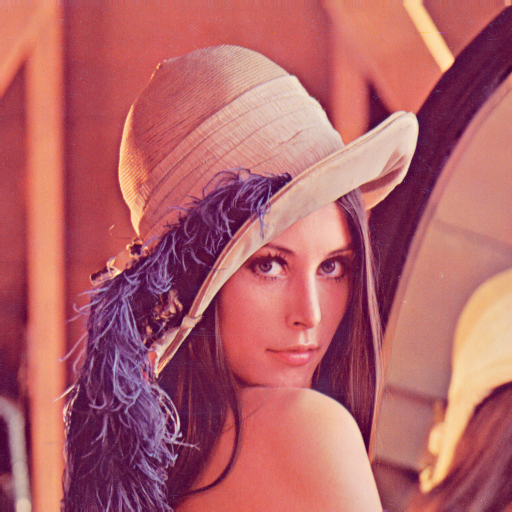
\includegraphics[width=0.4\textwidth,angle=90]{Images/lena}    &
		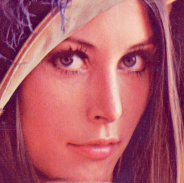
\includegraphics[width=0.4\textwidth]{Images/lenaCrop}    \\
	\end{tabular}
	\caption{Original image, scaling, rotation and cropping of the image}\label{img:Herausforderungen}
\end{figure}



\subsection{Representation of Images}

For a computer programme, an image is a matrix of numbers. The type of matrix is determined by the resolution, the number of colours and the colour depth. The resolution is the pair of values of how many elements, called pixels, the matrix has in height and in width. A simple example is shown in the image. The image has a resolution of 10 pixels in width and in height. The values can be either 0 or 1; in this illustration the value 0 represents the colour black, 0 the colour white.


\begin{figure}
	\begin{center}
		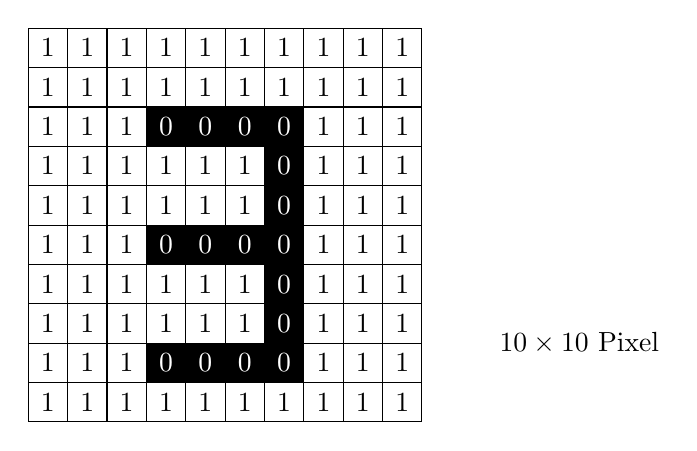
\begin{tikzpicture}
			
			%        \only<5->
			{
				\foreach \j in {0.5,1,...,5} 
				{
					\foreach \i in {0.5,1,...,5} {
						
						\node (P1) at (\i-0.25,\j-0.25) {1};
					}
				}
			}
			
			\draw[step=0.5,black,thin] (0,0) grid (5,5);
			
			%        \only<2->
			{
				
				\draw[fill=black] (1.5,0.5)  -- (2,0.5) -- (2,1) -- (1.5,1) -- cycle;
			}
			%        \only<3->
			{
				
				\draw[fill=black] (1.5,0.5)  -- (3.5,0.5) -- (3.5,1) -- (1.5,1) -- cycle;
				\draw[fill=black] (3,1)  -- (3.5,1) -- (3.5,4) -- (3,4) -- cycle;
				\draw[fill=black] (1.5,2)  -- (3.5,2) -- (3.5,2.5) -- (1.5,2.5) -- cycle;
				\draw[fill=black] (1.5,3.5)  -- (3.5,3.5) -- (3.5,4) -- (1.5,4) -- cycle;
			}
			
			%        \only<4->
			{
				\node (P1) at (1.75,0.75) {\textcolor{white}{0}};
				\node (P1) at (2.25,0.75) {\textcolor{white}{0}};
				\node (P1) at (2.75,0.75) {\textcolor{white}{0}};
				\node (P1) at (3.25,0.75) {\textcolor{white}{0}};
				\node (P1) at (3.25,1.25) {\textcolor{white}{0}};
				\node (P1) at (3.25,1.75) {\textcolor{white}{0}};
				\node (P1) at (3.25,2.25) {\textcolor{white}{0}};
				\node (P1) at (3.25,2.75) {\textcolor{white}{0}};
				\node (P1) at (3.25,3.25) {\textcolor{white}{0}};
				\node (P1) at (3.25,3.75) {\textcolor{white}{0}};
				
				\node (P1) at (1.75,2.25) {\textcolor{white}{0}};
				\node (P1) at (2.25,2.25) {\textcolor{white}{0}};
				\node (P1) at (2.75,2.25) {\textcolor{white}{0}};
				
				\node (P1) at (1.75,3.75) {\textcolor{white}{0}};
				\node (P1) at (2.25,3.75) {\textcolor{white}{0}};
				\node (P1) at (2.75,3.75) {\textcolor{white}{0}};
			}
			
			%        \only<6->
			{
				\node (Pixel) at (7,1) {$10 \times 10$ Pixel};
			}      
			
		\end{tikzpicture}
	\end{center}    
	
	
	\caption{Structure of a black and white image with $10 \times 10$ pixels}\label{img:schwarzweiss}
\end{figure}


Typical resolutions for camera images are recorded in the table. A pixel is defined by the number of colours and the colour depth. The colour depth indicates the range of values taken from the individual elements. These are usually integer values, specified in bits. Thus, an 8-bit value corresponds to a number between 0 and 255. A pixel can now contain such a numerical value for each colour. Often, however, a separate matrix is used for each colour. If one works with the RGB representation, one has the colours red, green and blue. The colour impression is obtained by superimposing the three images. The situation is shown in the figure. 



\begin{table}
	\centering
	\begin{tabular}{lcc}
		Resolution &=& width $\times$ height \\
		VGA             &=& $640 \times 480$ \\
		HD              &=& $1280 \times 720$\\
		Full HD         &=& $1920 \times 1080$\\
		4K               &=& $3840 \times 2160$\\
	\end{tabular}
	\caption{Standard resolutions of camera images}\label{Bild:Aufloesung}  	
\end{table}

\bigskip



\begin{figure}
	\centering
	\begin{tikzpicture}
		\node (P1) at (0,0) {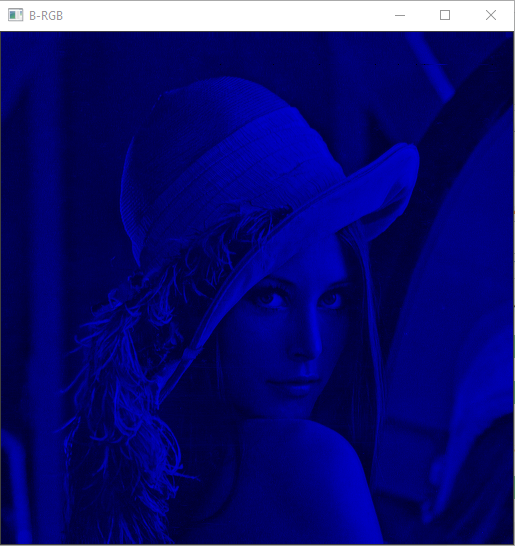
\includegraphics[width=0.2\textwidth]{Images/LenaBlue}};
		\node (P1) at (2,0) {$+$};
		\node (P1) at (4,0) {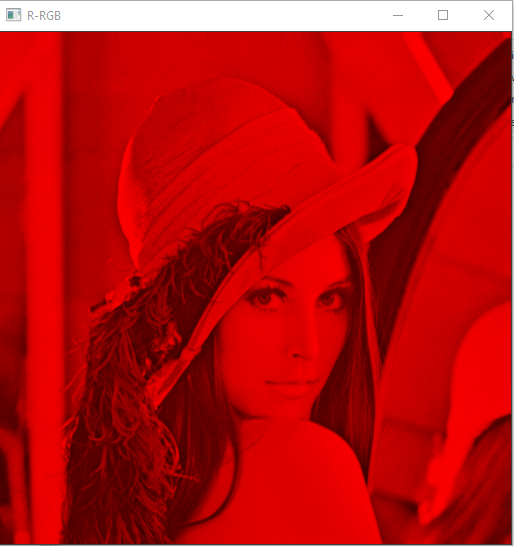
\includegraphics[width=0.2\textwidth]{Images/LenaRed}};
		\node (P1) at (6,0) {$+$};
		\node (P1) at (8,0) {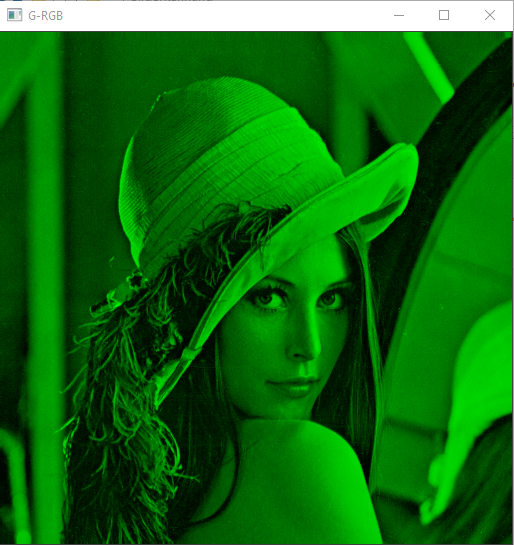
\includegraphics[width=0.2\textwidth]{Images/LenaGreen}};
		\node (P1) at (10,0) {$=$};
		\node (P1) at (12,0) {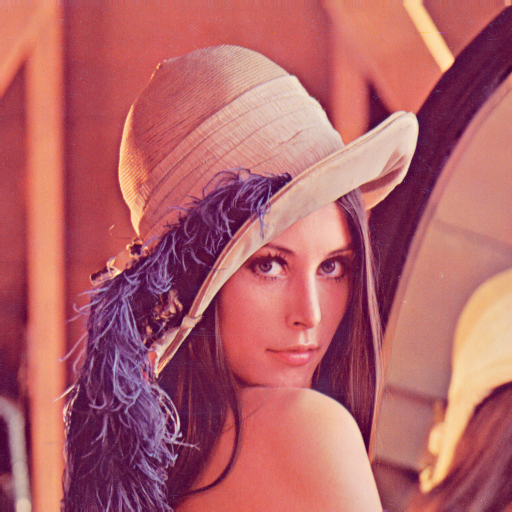
\includegraphics[width=0.2\textwidth]{Images/lena}};
	\end{tikzpicture}
	\caption{Image with 3 colour channels}\label{Bild:lenaRGB}
\end{figure}

Often greyscales are used instead of colour images. For this purpose, 256 greyscales are often used.% according to Figure~\ref{Image:256Greyscales}. 
When converting a colour image with three colours, the three matrices are added weighted. It has been shown that equal weighting of the colour channels is inappropriate. The OpenCV library for processing images uses the following weighting \cite{OpenCV:2020b}:

% Source: https://latexref.xyz/_005cincludegraphics.html
$$0.299 \cdot \hbox{Red} +0.587 \cdot \hbox{Green} +0.114 \cdot \hbox{Blue}$$

The conversion can be applied to the image \glqq Lena \grqq{}; this is in the figure. Other weights are used depending on the application. 
The above weights are empirically determined and are proportional to the sensitivity of the human eye to each of the trichromatic colours. The image has a colour depth of 8-bit. Other colour depths can also be used. A black and white image has the lowest colour depth. 

\begin{figure}[!h]
	\begin{center}
		
		%\begin{subfigure}[h]{0.4\linewidth}
		%todo Eigene Bilder    
		\includegraphics[width=0.7\textwidth]{Images/graylena}
		
		\caption{Greyscale with a value range from 0 to 255}\label{Bild:lenaGray}
	\end{center}    
\end{figure}




\begin{figure}[!h]
	\begin{center}
		
		%\begin{subfigure}[h]{0.4\linewidth}
		%todo Eigene Bilder    
		
		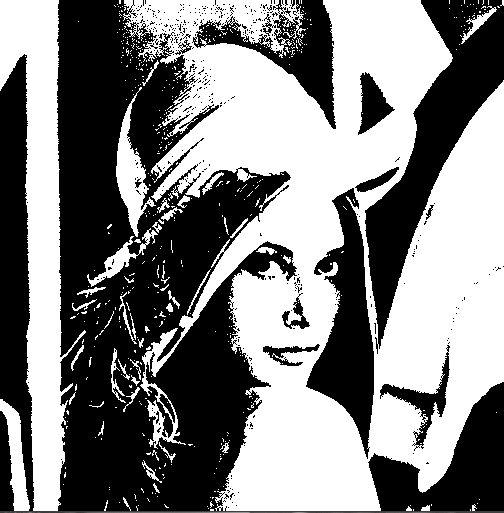
\includegraphics[width=0.3\textwidth]{Images/lenaBlackWhite126}
		\quad
		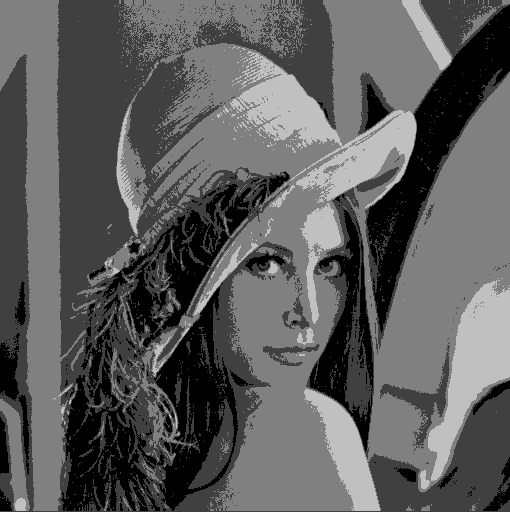
\includegraphics[width=0.3\textwidth]{Images/Grayscale4}
		\quad
		\includegraphics[width=0.3\textwidth]{Images/graylena}
		
		\caption{Black and white image, image with 4 grey levels and with 256 grey levels.}\label{Bild:}
	\end{center}    
\end{figure}


However, the quality of the image does not only depend on the parameters mentioned. The sharpness of the image also contributes to it. However, there is unfortunately no simple definition here, but is often shaped by subjective perception. On the other hand, it is possible to influence image sharpness by mathematical operations.  Blurring of an image can be achieved by blurring. 
Each pixel value is thereby represented by the average of the pixel values in a small window centred on the pixel. 

The resolution of the image affects the amount of computation required. For an image with a resolution of $674 \times 1200$ and a window size of $101 \times 101$, the new pixel value must be calculated separately for all three colour channels. In total this results in

$$674 \cdot 1200 \cdot 101 \approx 8.2 \cdot 10^9$$

operations. An example is shown in the figure with a filter size $5 \times 5$.


\begin{figure}
	\centering
	
	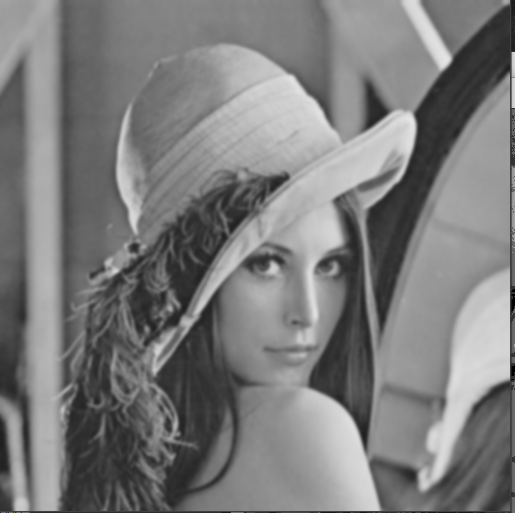
\includegraphics[width=0.3\textwidth]{Images/lenaBlurring}
	
	\caption{Softened image with a $5 \times 5$ filter}\label{Bild:Blurring}
\end{figure}


Another possibility of image processing is edge detection. With edge detection, the goal is to identify regions of the image where intensities of colour differ greatly. This is used to delineate objects and for object recognition. An example is given in Figure.

\begin{figure}
	\centering
	
	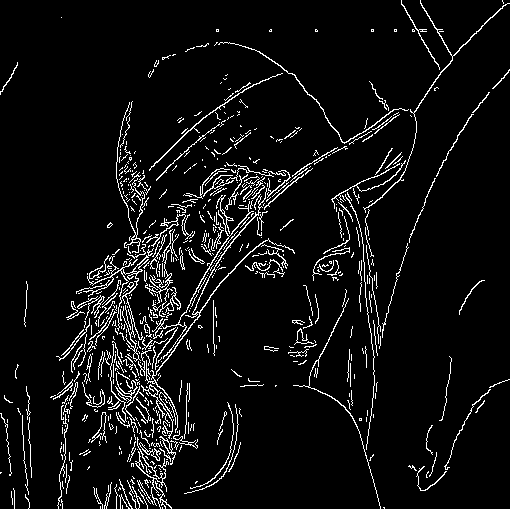
\includegraphics[width=0.3\textwidth]{Images/lenaBlackWhite}
	
	\caption{Edge detection on an image}\label{Bild:Kanten}
\end{figure}


\subsection{Convolution Neural Network Applications}

One focus for machine learning is the interpretation of images. Two cases must be distinguished here

\begin{enumerate}
	\item Object detection\index{Object detection}
	\item Image classification.\index{Image classification}
	
\end{enumerate}. 

When detecting objects, an image is examined to see if one or more objects can be identified. If an object is detected, the coordinates of the surrounding rectangle and the class or classes of the object are returned with a respective probability. With the segmentation\index{segmentation}, instead of the coordinates of the surrounding rectangle, a polygon course is returned that surrounds the object. In contrast, when classifying an image, a description of the image is searched for. In both cases CNN are commonly used and are described in the following section. 

A CNN expects an image as input information. If images do not contain colour information, they are represented as matrices whose number of columns and rows correspond to the number of pixels in width and height. In the case that an image contains colour information, such a matrix is created for each colour. In this case, one speaks of colour channel or simply of channel{index{channel}.
	
	
	CNN is a commonly used shift-invariant method for extracting adaptive features. Its success has contributed to the popularity of machine learning. In its history, its architectures have undergone a great evolution.\index{Alom:2018} Some well-known architectures are now described.    
	
	\subsection{CNN Architectures}
	
	
	\subsection*{LeNet\index{LeNet}}
	
	In 1998, the CNN architecture LeNet was the first CNN architecture to use back-propagation for practical applications. It thus transported Deep Learning from theory to practice. LeNet was used for handwritten digit recognition and was able to outperform all other existing methods. The architecture was very simple with only 5 layers consisting of $5\times 5$ convolutions and $2\times 2$ max-pooling, but paved the way for better and more complex models. \cite{LeCun:1998} The listing of elements in Table contains several points that will be described later.
	
	\begin{table}
		\begin{tabular}{ccc ccc c}
			\multicolumn{2}{c}{\textbf{Layer}} & \textbf{\begin{tabular}{c}Feature\\ Map \end{tabular}} & \textbf{Size} & \textbf{\begin{tabular}{c} Kernel \\Size\\ \end{tabular}} & \textbf{Stride} & \textbf{\begin{tabular}{c}Acti- \\vation \\function \end{tabular}}  \\ \hline
			Input   & Image            &   1 & $32\times 32$ &            - & - & - \\
			1        & Convolution     &   6 & $28\times 28$ &  $5\times 5$ & 1 & $\tanh$ \\  
			2        & \begin{tabular}{c}Average\\ Pooling  \end{tabular} &   6 & $14\times 14$ &  $2\times 2$ & 2 & $\tanh$ \\  
			3        & Convolution     &  16 & $10\times 10$ &  $5\times 5$ & 1 & $\tanh$ \\  
			4        & \begin{tabular}{c}Average\\ Pooling  \end{tabular} &  16 &   $5\times 5$ &  $2\times 2$ & 2 & $\tanh$ \\  
			5        & Convolution     & 120 &   $1\times 1$ &  $5\times 5$ & 1 & $\tanh$ \\  
			6        & \begin{tabular}{c}Neural\\ Network  \end{tabular} &   - &          $84$ &    -         & - & $\tanh$ \\  
			Ausgabe  & \begin{tabular}{c}Neural\\ Network  \end{tabular}  &   - &          $10$ &    -         & - & softmax \\  
		\end{tabular}  		
		\caption{Structural elements of LeNet}
		
	\end{table}
	
	
	
	
	\subsection*{AlexNet\index{AlexNet}} 
	
	The AlexNet architecture was the first to use CNN models implemented on GPUs .  In 2012, this really connected the growing computing power with Deep Learning. AlexNet is significantly deeper and more complex than LeNet They also started using ReLU activations instead of sigmoid or tanh, which helped train better models. AlexNet not only won the 2012 ImageNet classification competition, but beat the runner-up by a margin that suddenly made non-neural models almost obsolete. \cite{Krizhevsky:2012}
	
	
	
	\subsection*{InceptionNet\index{InceptionNet}}
	
	
	The architecture InceptionNet\index{InceptionNet} used the increased possibilities of the hardware. The architecture was again much deeper and richer in parameters than the existing models. To deal with the problem of training deeper models, they used the idea of multiple auxiliary classifiers present between the model to prevent the gradient from breaking. One of their ideas was to use kernels of different sizes in parallel, thus increasing the width of the model instead of the depth. This allows such an architecture to extract both larger and smaller features simultaneously. \cite{Szegedy:2014}
	
	
	\subsection*{VGG\index{VGG}}
	
	Many architectures tried to achieve better results by using larger convolution kernels. For example, the architecture AlexNet\index{AlexNet} uses cores of size $11 \times 11$, among others. The architecture VGG\index{VGG} took the path of using several cores of size $3\times 3$ in succession and more non-linearities in the form of activation functions. This again improved the results. \cite{Zhang:2015,Simonyan:2015}
	
	\subsection*{Residual Neural Network (ResNet)\index{ResNet}}
	
	The deeper the architectures became, the more often the problem occurred during training that the amount of the gradient became too small. The backpropagation\index{backpropagation} then aborted and the parameters could not be determined. In the RESNETs architecture, to prevent the problem, residual or shortcut links were introduced to create alternative paths for the gradient to skip the middle layers and directly reach the initial layers. In this way, the authors were able to train extremely deep models that previously did not perform well. It is now common practice to have residual connections in modern CNN architectures. \cite{He:2016}
	
	
	
	
	\subsection*{MobileNet \& MobileNetV2\index{MobileNet}\index{MobileNetV2}} 
	
	The MobileNet architecture is designed for edge computers and smart phones that are limited in memory and computing power. This has opened up a large field of new applications. This is in contrast to the previous strategy of increasing the size of architectures by introducing separable convolutions. In simple terms, a two-dimensional convolutional kernel is split into two separate convolutions, namely the depth convolution, which is responsible for collecting the spatial information for each individual channel, and the point convolution, which is responsible for the interaction between the different channels. Later, MobileNetV2 was also introduced with residual connections and other optimisations in the architecture to further reduce the model size. \cite{Howard:2017,MobileNet:2018}
	
	\subsection*{EfficientNet\index{EfficientNet}} 
	The architecture is the result of considering that the various architectures to date, focus on either performance or computational efficiency. The authors of \cite{Tan:2020} claimed that these two problems can be solved by similar architectures. They proposed a common CNN skeleton architecture and three parameters, namely the width, the depth and the resolution. The width of the model refers to the number of channels present in the different layers, the depth refers to the number of layers in the model and the resolution refers to the size of the input image to the model. They claimed that by keeping all these parameters small, one can create a competitive yet computationally efficient CNN model. On the other hand, by increasing the value of these parameters, one can create a model that is designed for accuracy.
	
	
	\subsection{General Structure}
	
	
	
	In the description of the architectures, some elements necessary for the construction were mentioned. All building blocks can be listed as follows:
	
	\begin{itemize}
		\item Convolutional layer (convolution)
		\item Activation function
		\item Pooling
		\item Flattening
		\item Neural network
	\end{itemize}
	
	Each component is characterised by further variables. The combination and configuration of the building blocks are summarised in the so-called hyperparameters. By specifying the hyperparameter\index{hyperparameter}, the architecture and the number of parameters is determined. For example, in a neural network, the hyperparameters\index{hyperparameters} are the number of layers, the number of neurons per layer and the determination of the activation functions. If the number of all neurons is now determined, this results in the number of parameters that are determined during the training.
	
	In the table~\ref{concept:Parameter} some architectures are compared. The table indicates the number of parameters to be trained.  If an image is classified, the models give different possibilities and assign a probability to them. The accuracy now indicates the percentage with which the image matches the prediction with the highest probability. For this purpose, the models were trained and validated with the ImageNet\index{ImageNet}. 
	
	
	
	
	\begin{table}
		\begin{tabular}{lllrc}
			Model             & Size   & Accuracy    & Parameter   & Depth \\ \hline
			VGG16             & 528 MB & 71{,}3\%    & 138.357.544 & 23 \\     
			VGG19             & 549 MB & 71{,}3\%    & 143.667.240 & 26 \\     
			ResNet-50         &  98 MB & 74{,}9\%    &  25.636.712 & 50 \\     
			ResNet-101        & 171 MB & 76{,}4\%    &  44.707.176 & 101 \\     
			ResNet-152        & 232 MB & 76{,}6\%    &  60.419.944 & 152 \\     
			InceptionV3       &  92 MB & 77{,}9\%    &  23,851,784 & 159 \\
			InceptionResNetV2 & 215 MB & 80{,}3\%    &  55,873,736 & 572 \\
			%     NASNetMobile      &  23 MB & 74{,}4\%    &   5.326.716 & --\\
			%     NASNetLarge       & 343 MB & 82{,}5\%    &  88.949.818 & --\\
			MobileNet         &  16 MB & 70,{4}\%    &   4.253.864 & 88 \\       
			MobileNetV2       &  14 MB & 71,{3}\%    &   3.538.984 & 88 \\       
		\end{tabular}
		\caption{Characteristics of different CNN architectures\index{VGG}\index{ResNet}\index{Inception}\index{MonileNet}}\label{concept:Parameter}
	\end{table}
	
	The individual building blocks are now described below.
	
	
	
	\subsection*{Input and Output}
	
	When a model receives an image as input, fields with pixel values are transferred. The height, the width and the number of colour channels determine the size of the fields. The elements of the fields then contain values between zero and 255. This value is the intensity of the pixel. The model then determines probabilities of how to classify an image based on these fields. For example, the result could be that $81\%$ of the image is a turtle, $11\%$ is a gun and $8\%$ is a chocolate bar.
	
	
	
	
	\subsection*{Convolution Layer}\label{subsec:conv2d}
	
	In a convolution layer, the input data is modified by one or more filters. In image processing, this is the application of a defined set of filters to two-dimensional data.
	
	The size of this filter is defined by the so-called kernel: a $3 \times 3$ kernel is represented by a $3 \times 3$ matrix. In order to be able to apply the filter, a range of pixel values is defined that has the same size; the pixel values are then also stored in a matrix. By convolution of the matrix, as shown in the equation Convolution Matrix, a value is assigned to the matrix and the filter. 
	
	
	\begin{figure}
		
		$$A \ast C 
		=
		\left(
		\begin{matrix}
			a_{11} & a_{12} & a_{13}\\
			a_{21} & a_{22} & a_{23}\\
			a_{31} & a_{32} & a_{33}\\
		\end{matrix}
		\right)
		\ast
		\left(
		\begin{matrix}
			c_{11} & c_{12} & c_{13}\\
			c_{21} & c_{22} & c_{23}\\
			c_{31} & c_{32} & c_{33}\\
		\end{matrix}
		\right)
		= 
		\sum_{i=1}^3\sum_{j=1}^3  a_{ij} \cdot c_{ij}
		$$
		
		\caption{Definition of the convolution of two matrices}\label{concept:FaltungMatrix}
		
	\end{figure}
	
	To apply a filter, matrices must therefore be systematically selected from the pixel values. Since the dimension of a kernel is defined by an odd number $2n+1$, a surrounding matrix can be assigned to each pixel value that has a distance greater than $n$ from the edge. In the figure~\ref{concept:conv2d} such a situation is shown. The filter, labelled $C$ and coloured purple, has a dimension of $3 \times 3$. In the matrix $A$, the field of pixel values, a region is coloured red. In the middle is the pixel from the fifth column and the second row. The filter is now applied to this area of the matrix $A$. The result is then entered into the matrix $A\ast C$. In this case the value is $4$ and marked green.
	
	
	A filter is now moved step by step over the data.  The filter can be applied to any pixel value that is far enough from the edge, or individual pixels can be skipped. This is defined by the step size, also called stride. With a step size of one, every pixel is used. To reduce the output size, stride sizes larger than one can be used; it is also possible to set different stride sizes for width and height. If a step size of $2$ is specified in both directions, the amount of data has been reduced to $25\%$. \cite{Dumoulin:2016}
	
	In the figure~\ref{concept:conv2d}, the input matrix is a $7\times 7$ matrix. Since a step size of one is applied here, the result is a $5\times 5$ matrix.
	
	Often an activation function is applied to each result.
	
	\begin{figure}[htb]
		
		
		\centering
		\begin{tikzpicture}
			\matrix (mtr) [matrix of nodes,row sep=-\pgflinewidth, nodes={draw}]
			{
				0 & 1 & 1 & |[fill=red!20]| 1 & |[fill=red!20]| 0 & |[fill=red!20]| 0 & 0\\
				0 & 0 & 1 & |[fill=red!20]| 1 & |[fill=red!20]| 1 & |[fill=red!20]| 0 & 0\\
				0 & 0 & 0 & |[fill=red!20]| 1 & |[fill=red!20]| 1 & |[fill=red!20]| 1 & 0\\
				0 & 0 & 0 & 1 & 1 & 0 & 0\\
				0 & 0 & 1 & 1 & 0 & 0 & 0\\
				0 & 1 & 1 & 0 & 0 & 0 & 0\\
				1 & 1 & 0 & 0 & 0 & 0 & 0\\
			};
			
			\draw[very thick, red!20] (mtr-1-4.north west) rectangle (mtr-3-6.south east);
			
			\node [below= of mtr-5-4.south] (lm) {$\mathbf{A}$};
			
			\node[right = 0.2em of mtr] (str) {$*$};
			
			\node (ast2) at (2,-2) {$\mathbf{*}$};
			\node (ast2) at (4,-2) {$\mathbf{=}$};
			
			\matrix (K) [right=0.2em of str,matrix of nodes,row sep=-\pgflinewidth, nodes={draw, fill=blue!20}]
			{
				1 & 0 & 1 \\
				0 & 1 & 0 \\
				1 & 0 & 1 \\
			};
			\node [below = of K-3-2.south] (lk) {$\mathbf{C}$};
			
			\node [right = 0.2em of K] (eq) {$=$};
			
			\matrix (ret) [right=0.2em of eq,matrix of nodes,row sep=-\pgflinewidth, nodes={draw}]
			{
				1 & 4 & 3 & |[fill=green!20]| 4 & 1\\
				1 & 2 & 4 & 3 & 3\\
				1 & 2 & 3 & 4 & 1\\
				1 & 3 & 3 & 1 & 1\\
				3 & 3 & 1 & 1 & 0\\
			};
			\node [below = of ret-4-3.south] (lim) {$\mathbf{A} \ast  \mathbf{C}$};
			
			\draw[very thick, green!20] (ret-1-4.north west) rectangle (ret-1-4.south east);
			
			\draw[densely dotted, blue!30, thick] (mtr-1-4.north west) -- (K-1-1.north west);
			\draw[densely dotted, blue!30, thick] (mtr-3-4.south west) -- (K-3-1.south west);
			\draw[densely dotted, blue!30, thick] (mtr-1-6.north east) -- (K-1-3.north east);
			\draw[densely dotted, blue!30, thick] (mtr-3-6.south east) -- (K-3-3.south east);
			
			\draw[densely dotted, green!30, thick] (ret-1-4.north west) -- (K-1-1.north west);
			\draw[densely dotted, green!30, thick] (ret-1-4.south west) -- (K-3-1.south west);
			\draw[densely dotted, green!30, thick] (ret-1-4.north east) -- (K-1-3.north east);
			\draw[densely dotted, green!30, thick] (ret-1-4.south east) -- (K-3-3.south east);
			
			\matrix (K) [right=0.2em of str,matrix of nodes,row sep=-\pgflinewidth, nodes={draw, fill=blue!20}]
			{
				1 & 0 & 1 \\
				0 & 1 & 0 \\
				1 & 0 & 1 \\
			};
			
			\draw[very thick, blue!20] (K-1-1.north west) rectangle (K-3-3.south east);
			
			\node[anchor=south east, inner sep=0.01em, blue!20] at (mtr-1-4.south east) (xx) {\scalebox{.5}{$\times 1$}};
			\node[anchor=south east, inner sep=0.01em, blue!20] at (mtr-1-5.south east) (xx) {\scalebox{.5}{$\times 0$}};
			\node[anchor=south east, inner sep=0.01em, blue!20] at (mtr-1-6.south east) (xx) {\scalebox{.5}{$\times 1$}};
			\node[anchor=south east, inner sep=0.01em, blue!20] at (mtr-2-4.south east) (xx) {\scalebox{.5}{$\times 0$}};
			\node[anchor=south east, inner sep=0.01em, blue!20] at (mtr-2-5.south east) (xx) {\scalebox{.5}{$\times 1$}};
			\node[anchor=south east, inner sep=0.01em, blue!20] at (mtr-2-6.south east) (xx) {\scalebox{.5}{$\times 0$}};
			\node[anchor=south east, inner sep=0.01em, blue!20] at (mtr-3-4.south east) (xx) {\scalebox{.5}{$\times 1$}};
			\node[anchor=south east, inner sep=0.01em, blue!20] at (mtr-3-5.south east) (xx) {\scalebox{.5}{$\times 0$}};
			\node[anchor=south east, inner sep=0.01em, blue!20] at (mtr-3-6.south east) (xx) {\scalebox{.5}{$\times 1$}};	
		\end{tikzpicture}
		\caption{Convolution layer with $3 \times 3$ kernel and stride (1, 1)}
		\label{concept:conv2d}
		
	\end{figure}
	
	When defining the filters, make sure that the filter is defined for each channel.
	To capture the features in an image, the values in the filter must match the structure of the original pixel values of the image. Basically, if there is a shape in the input image that generally resembles the curve that this filter represents, then the convolution will result in a large value.
	
	As a rule, several filters are used in parallel. The result is so-called feature maps\index{feature maps}. Further convolution layers are then applied to this result, which in turn generate feature maps. 
	
	
	\subsection{Feature Identification}
	
	A convolution is defined by filters. Each filter can be interpreted as an identifier of features. Features are, for example, edges, colours or even curves. For example, the $7\times 7$ filter is considered:
	
	$$\left(
	\begin{array}{ccc ccc c}
		0 & 0 & 0 &  0 & 0  & 50 & 0 \\
		0 & 0 & 0 &  0 & 50 &  0 & 0 \\
		0 & 0 & 0 & 50 &  0 &  0 & 0 \\
		0 & 0 & 0 & 50 &  0 &  0 & 0 \\
		0 & 0 & 0 & 50 &  0 &  0 & 0 \\
		0 & 0 & 0 & 50 &  0 &  0 & 0 \\
		0 & 0 & 0 &  0 &  0 &  0 & 0 \\
	\end{array}
	\right)
	$$  
	
	This filter can also be visualised as images:
	
	
	
	To demonstrate the effect of the filter, a sample image~\ref{concept:FilterCat} is considered:
	
	
	\begin{figure}
		\centering    
		
		
\includegraphics[scale=0.3]{Images/cat}
		
		\caption{Beispielanwendung für einen Filter und ein Ausschnitt}\label{concept:FilterCat}
	\end{figure}
	
	In the example image~\ref{concept:FilterCat} a section is marked to which the filter is applied. 
	
	
	
	$$
	\left(
	\begin{array}{ccc ccc c}
		0 & 0 & 0 &  0 & 0  &  0 & 30 \\
		0 & 0 & 0 &  0 & 80 & 80 & 80 \\
		0 & 0 & 0 & 30 & 80 &  0 &  0 \\
		0 & 0 & 0 & 80 & 80 &  0 &  0 \\
		0 & 0 & 0 & 80 & 80 &  0 &  0 \\
		0 & 0 & 0 & 80 & 80 &  0 &  0 \\
		0 & 0 & 0 & 80 & 80 &  0 &  0 \\
	\end{array}
	\right)
	\star
	\left(
	\begin{array}{ccc ccc c}
		0 & 0 & 0 &  0 & 0  & 50 & 0 \\
		0 & 0 & 0 &  0 & 50 &  0 & 0 \\
		0 & 0 & 0 & 50 &  0 &  0 & 0 \\
		0 & 0 & 0 & 50 &  0 &  0 & 0 \\
		0 & 0 & 0 & 50 &  0 &  0 & 0 \\
		0 & 0 & 0 & 50 &  0 &  0 & 0 \\
		0 & 0 & 0 &  0 &  0 &  0 & 0 \\
	\end{array}
	\right)$$
	
	$$
	=
	\left(
	\begin{array}{ccc ccc c}
		0 & 0 & 0 &  0 & 0  &  0 & 30 \\
		0 & 0 & 0 &  0 & 80 & 80 & 80 \\
		0 & 0 & 0 & 30 & 80 &  0 &  0 \\
		0 & 0 & 0 & 80 & 80 &  0 &  0 \\
		0 & 0 & 0 & 80 & 80 &  0 &  0 \\
		0 & 0 & 0 & 80 & 80 &  0 &  0 \\
		0 & 0 & 0 & 80 & 80 &  0 &  0 \\
	\end{array}
	\right)
	$$  
	
	The basic property of filters is clarified. If there is a shape in the input image that generally resembles the filter, then large values result. A probability is then assigned via the activation function. Various filters are then defined and applied in the convolution layer. The result is then the feature map. The figure shows some examples of concrete visualisations of filters of the first convolutional layer of a trained network. 
	
	
	\subsection{Edge Detection}
	
	Suitable filters can also be defined for edge detection. The filter
	
	
	$$\left(
	\begin{array}{ccc}
		1 & 0 & -1 \\
		1 & 0 & -1 \\
		1 & 0 & -1 \\
	\end{array}
	\right)
	$$
	
	can be used for a vertical edge detection, whereas the filter 
	
	
	$$\left(
	\begin{array}{ccc}
		1 &  1 &  1 \\
		0 &  0 &  0 \\
		-1 & -1 & -1 \\
	\end{array}
	\right)
	$$
	
	can be used for a horizontal one. Both filters are now applied to a vertical edge.
	
	
	\begin{figure}
		$$
		\left(
		\begin{array}{ccc ccc}
			10 & 10 & 10 & 0 & 0 & 0 \\
			10 & 10 & 10 & 0 & 0 & 0 \\
			10 & 10 & 10 & 0 & 0 & 0 \\
			10 & 10 & 10 & 0 & 0 & 0 \\
			10 & 10 & 10 & 0 & 0 & 0 \\
			10 & 10 & 10 & 0 & 0 & 0 \\
		\end{array}
		\right)
		\ast
		\left(
		\begin{array}{ccc}
			1 & 0 & -1 \\
			1 & 0 & -1 \\
			1 & 0 & -1 \\
		\end{array}
		\right)
		=
		\left(
		\begin{array}{cccc}
			0 & 30 & 30 & 0 \\
			0 & 30 & 30 & 0 \\
			0 & 30 & 30 & 0 \\
			0 & 30 & 30 & 0 \\
		\end{array}
		\right)
		$$
		
		$$
		\left(
		\begin{array}{ccc ccc}
			10 & 10 & 10 & 0 & 0 & 0 \\
			10 & 10 & 10 & 0 & 0 & 0 \\
			10 & 10 & 10 & 0 & 0 & 0 \\
			10 & 10 & 10 & 0 & 0 & 0 \\
			10 & 10 & 10 & 0 & 0 & 0 \\
			10 & 10 & 10 & 0 & 0 & 0 \\
		\end{array}
		\right)
		\ast
		\left(
		\begin{array}{ccc}
			1 &  1 &  1 \\
			0 &  0 &  0 \\
			-1 & -1 & -1 \\
		\end{array}
		\right)
		=
		\left(
		\begin{array}{cccc}
			0 & 0 & 0 & 0 \\
			0 & 0 & 0 & 0 \\
			0 & 0 & 0 & 0 \\
			0 & 0 & 0 & 0 \\
		\end{array}
		\right)
		$$
		\caption{Detection of vertical and horizontal edges}
	\end{figure}
	
	Edges can be present in any arrangement in images, edge detection must take this into account. That is, if a CNN is trained, the filters evolve based on the given images. 
	
	
	
	\subsection*{Padding}
	
	In the previous representation, filters could not be applied to boundary values. On the one hand, this means that information is not used, on the other hand, the size of the images is reduced each time the folding is applied. To prevent this, padding is applied. For a filter of dimension $(2n+1) \times (2m+1)$, the input image is padded with an additional border of size
	$n$ and $m$. The additional values are each zero occupied.
	
	
	
	\subsection*{Activation function}\label{subsec:activation}
	
	The activation function is applied to the respective output of a layer and determines how the output value should be interpreted by applying a defined function. Here, the respective input values, as well as a bias, are included in the calculation and determine whether the neuron is triggered \cite{Nwankpa:2018}. In this example, the ReLU function is used for this: for input values less than or equal to zero, the function returns zero; for positive values, it behaves linearly \cite{Agarap:2018}. Thus, only positive values are returned (\ref{fig:relu}).
	
	\begin{figure}
		\centering
		\begin{tikzpicture}
			\begin{axis}[
				domain=-5:5,
				axis equal,
				xmin=-5,
				xmax=5,
				axis y line=middle,
				axis x line=center,
				axis line style={->},
				xlabel={$x$},
				ylabel={$y$},
				xtick={-5,...,5},
				ytick={0,...,5},]
				\addplot+[mark=none,red,domain=-5:0] {0};
				\addplot+[mark=none,red,domain=0:5] {x};
			\end{axis}
		\end{tikzpicture}
		\caption{Representation of the ReLu activation function}
		\label{fig:relu}
	\end{figure}
	
	\subsection*{Pooling}
	
	
	After the use of convolutional layers, pooling layers are often used in CNN to reduce the size of the representation, to also speed up the calculations as well as to make some of the detection functions a bit more robust. A distinction is usually made between two pooling methods.
	
	\begin{itemize}
		\item Max Pooling
		\item Average Pooling
	\end{itemize}
	
	In pooling, areas of a matrix are combined. The ranges are defined by two values $n$ and $m$. The ranges are submatrices of the matrix of size $n \times m$. A function is then applied to each submatrix.
	
	In max-pooling, the maximum value of the submatrix is determined and entered as the result. In the case of average pooling, the average value of the matrix elements is determined instead of the maximum value and used further.
	
	
	In the case of pooling, a window with a defined size is moved over the input matrix and the corresponding value within the window is taken over as a pooled value. The step size with which the window moves over the matrix is defined via a parameter \cite{Dumoulin:2016}. The default value corresponds to the size of the sub-matrix. An example is shown in the representation~\ref{fig:maxpooling2d}: a 4x4 matrix is defined with size \PYTHON{pool\_size}  2x2and a step size \PYTHON{stride\_size} 2x2 processed. Since two values are combined into each dimension, the dimensions of the output matrix are halved in contrast to the input matrix. \cite{Britz:2015}
	
	\begin{figure}[htb]
		\centering
		
		\def\yspacing{.75em}
		\begin{tikzpicture}[auto, node distance=0cm,>=latex']
			% Root folder blocks
			% Subfolder Blocks
			\node [smallblock] (bin) {2};
			\node [smallblock, below=of bin] (bin2) {0};
			\node [smallblock, right=of bin] (bin3) {0};
			\node [smallblock, right=of bin2] (bin4) {1};
			
			\node [smallblock, fill=blue!20, right=of bin3] (bin5) {1};
			\node [smallblock, fill=blue!20, below=of bin5] (bin6) {0};
			\node [smallblock, fill=blue!20, right=of bin5] (bin7) {1};
			\node [smallblock, fill=blue!20, right=of bin6] (bin8) {0};
			
			\node [smallblock, fill=green!20, below=of bin2] (bin9) {0};
			\node [smallblock, fill=green!20, below=of bin9] (bin10) {0};
			\node [smallblock, fill=green!20, right=of bin9] (bin11) {0};
			\node [smallblock, fill=green!20, right=of bin10] (bin12) {3};
			
			\node [smallblock, fill=yellow!20, right=of bin11] (bin13) {1};
			\node [smallblock, fill=yellow!20, below=of bin13] (bin14) {0};
			\node [smallblock, fill=yellow!20, right=of bin13] (bin15) {0};
			\node [smallblock, fill=yellow!20, right=of bin14] (bin16) {0};
			
			\node [smallblock, right=of bin8.east, xshift=10em] (res1) {2};
			\node [smallblock, fill=green!20, below=of res1] (res2) {3};
			\node [smallblock, fill=blue!20, right=of res1] (res3) {1};
			\node [smallblock, fill=yellow!20, right=of res2] (res4) {1};
			
			\draw [arrow] (bin8.south east)++(1em, 0) -- ($(res1.south west)+(-1em,0)$) node[midway, sloped, above] {\footnotesize pool\_size = (2,2)} node[midway, sloped, below] {\footnotesize stride = (2,2)};
		\end{tikzpicture}
		
		\bigskip
		
		\def\yspacing{.75em}
		\begin{tikzpicture}[auto, node distance=0cm,>=latex']
			% Root folder blocks
			% Subfolder Blocks
			\node [smallblock] (bin) {2};
			\node [smallblock, below=of bin] (bin2) {0};
			\node [smallblock, right=of bin] (bin3) {0};
			\node [smallblock, right=of bin2] (bin4) {1};
			
			\node [smallblock, fill=blue!20, right=of bin3] (bin5) {1};
			\node [smallblock, fill=blue!20, below=of bin5] (bin6) {0};
			\node [smallblock, fill=blue!20, right=of bin5] (bin7) {1};
			\node [smallblock, fill=blue!20, right=of bin6] (bin8) {0};
			
			\node [smallblock, fill=green!20, below=of bin2] (bin9) {0};
			\node [smallblock, fill=green!20, below=of bin9] (bin10) {0};
			\node [smallblock, fill=green!20, right=of bin9] (bin11) {0};
			\node [smallblock, fill=green!20, right=of bin10] (bin12) {3};
			
			\node [smallblock, fill=yellow!20, right=of bin11] (bin13) {1};
			\node [smallblock, fill=yellow!20, below=of bin13] (bin14) {0};
			\node [smallblock, fill=yellow!20, right=of bin13] (bin15) {0};
			\node [smallblock, fill=yellow!20, right=of bin14] (bin16) {0};
			
			\node [smallblock, right=of bin8.east, xshift=10em] (res1) {0{,}75};
			\node [smallblock, fill=green!20, below=of res1] (res2) {0{,}50};
			\node [smallblock, fill=blue!20, right=of res1] (res3) {0{,}75};
			\node [smallblock, fill=yellow!20, right=of res2] (res4) {0{,}25};
			
			\draw [arrow] (bin8.south east)++(1em, 0) -- ($(res1.south west)+(-1em,0)$) node[midway, sloped, above] {\footnotesize pool\_size = (2,2)} node[midway, sloped, below] {\footnotesize stride = (2,2)};
		\end{tikzpicture}
		
		\caption{Application of max-pooling and average-pooling}
		\label{fig:maxpooling2d}
		
	\end{figure}
	
	
	\subsection*{Flattening}\label{subsec:flatten}
	
	With a flatten layer, the multidimensional input object is converted into a vector. For example, if an object with dimensions 5x7x7 is passed in, it results in a one-dimensional vector with 245 elements. In the figure~\ref{fig:flatten}, the function Flatten is applied to a $3 \times 3$ matrix. The function is used when a neural network is subsequently used.
	
	\begin{figure}[htb]
		\centering
		
		\def\yspacing{.75em}
		\begin{tikzpicture}[auto, node distance=0cm,>=latex']
			% Root folder blocks
			% Subfolder Blocks
			\node [smallblock] (bin) {1};
			\node [smallblock, right=of bin] (bin2) {1};
			\node [smallblock, right=of bin2] (bin3) {0};
			
			\node [smallblock, fill=blue!20, below=of bin] (bin3) {4};
			\node [smallblock, fill=blue!20, right=of bin3] (bin4) {2};
			\node [smallblock, fill=blue!20, right=of bin4] (bin5) {1};
			
			\node [smallblock, fill=green!20, below=of bin3] (bin6) {0};
			\node [smallblock, fill=green!20, right=of bin6] (bin7) {2};
			\node [smallblock, fill=green!20, right=of bin7] (bin8) {1};
			
			\node [smallblock, right=of bin5, xshift=6em] (res1) {1};
			\node [smallblock, right=of res1] (res2) {1};
			\node [smallblock, right=of res2] (res3) {0};
			\node [smallblock, fill=blue!20, right=of res3] (res4) {4};
			\node [smallblock, fill=blue!20, right=of res4] (res5) {2};
			\node [smallblock, fill=blue!20, right=of res5] (res6) {1};
			\node [smallblock, fill=green!20, right=of res6] (res7) {0};
			\node [smallblock, fill=green!20, right=of res7] (res8) {2};
			\node [smallblock, fill=green!20, right=of res8] (res9) {1};
			
			\draw [arrow] (bin5.east)++(1em, 0) -- ($(res1.west)+(-1em,0)$);
		\end{tikzpicture}
		\caption{Application of flattening}
		\label{fig:flatten}
		
	\end{figure}
	
	\subsection*{Dense Layer}\label{subsec:dense}
	
	In a layer, or fully-connected layer, is a layer that uses a neural network. This means that each of the previous outputs are fed into each of the inputs of the layer. Similarly, each output is linked to each of the subsequent inputs. This type of layer is usually used to be able to classify using the feature maps generated by the convolution.  \cite{Keras:2020b} It is determined by the number of neurons and the associated activation function.
	
	
	
	\subsection*{Model used for a CIFAR 10 classification}\label{sec:usedmodel}
	
	The model used is an object \textbf{keras.models.Sequential}. With the help of the method add, the individual layers can be added to this model. The structure of the model is modelled on the Tensorflow tutorial for CNN \cite{GoogleTensorFlowCNN:2020}. The structure of the model is shown in \cref{fig:networklayers}.
	
	The layers described previously are now used to create a model for classifying the dataset CIFAR-10 with Keras. Here we look at how these layers are applied in the Python environment and how the size and dimension of the data changes between each layer. The dimensions of the input as well as output data of the individual layers are mapped in \cref{fig:networklayers}.
	
	\begin{lstlisting}[language=MyPython, numbers=left]
		MODEL = models.Sequential()
		MODEL.add(layers.Conv2D(filters=32, kernel_size=(3, 3), activation='relu', input_shape=(32, 32, 3)))
		MODEL.add(layers.MaxPooling2D(pool_size=(2, 2)))
		MODEL.add(layers.Conv2D(filters=64, kernel_size=(3, 3), activation='relu'))
		MODEL.add(layers.MaxPooling2D(pool_size=(2, 2)))
		MODEL.add(layers.Conv2D(filters=64, kernel_size=(3, 3), activation='relu'))
		MODEL.add(layers.Flatten())
		MODEL.add(layers.Dense(units=64, activation='relu'))
		MODEL.add(layers.Dense(units=10))
	\end{lstlisting}
	
	
	At the beginning, as described in , a Keras object \PYTHON{Sequential} is created. The first layer added to this model is a convolution layer \PYTHON{Conv2D}, see line 2. This is defined with 32 filters, each with a size of 3x3. If, when creating the object, the parameter stride is not explicitly specified when the object is created, the default step size (1, 1) is used. Since the input data into the model are RGB images with $32 \times 32$ pixels, see \cref{sec:dataset}, the parameter \PYTHON{input\_shape} is taken to be 32x32x3. This configuration transforms the input data in the first convolutional layer from 32x32x3 to an output of 30x30x32. A separate feature map is stored for each of the applied filters.
	
	The next layer, a max-pooling layer with a \PYTHON{pool\_size} of 2x2, reduces the data size from 30x30x32 to 15x15x32 (line 3).
	
	\begin{figure}[htb]
		\centering
		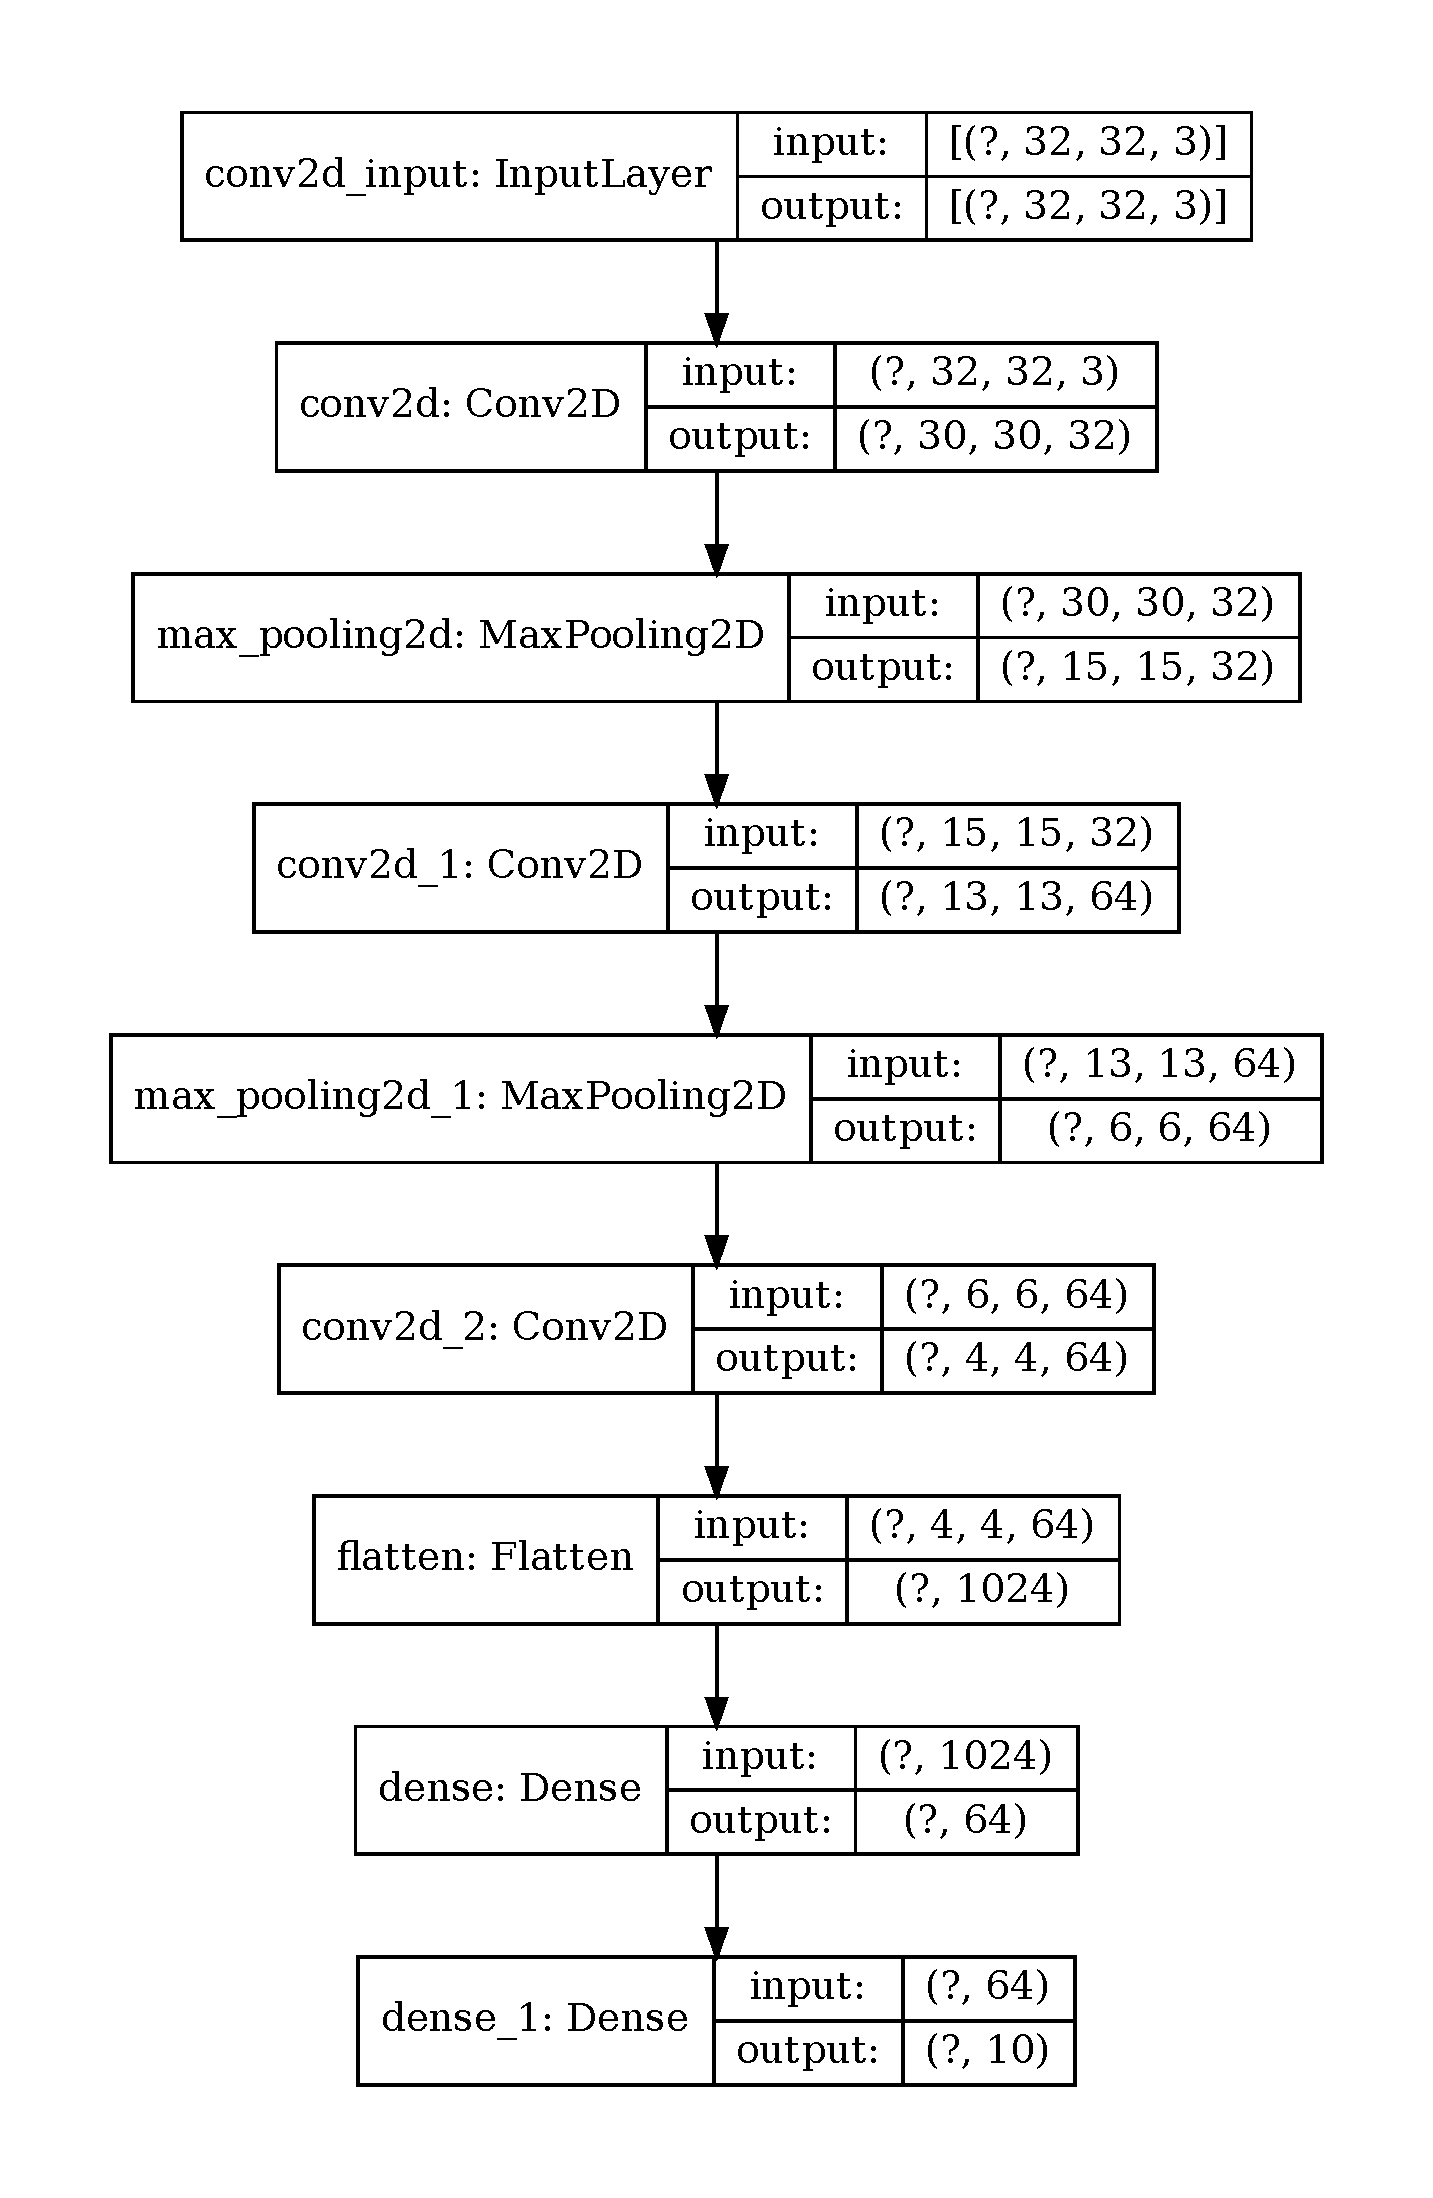
\includegraphics[trim = 0mm 19mm 0mm 19mm, clip, height=9cm]{Images/cifar-model-graph-detailed.pdf}
		\caption{Structure of the neural network used}
		\label{fig:networklayers}
	\end{figure}
	
	This data is now fed again into a convolutional layer, which here is also configured with a \PYTHON{kernel\_size} of 2x2, line 4, but with 64 filters. This transforms the data from 15x32 to 13x64.
	
	To reduce the amount of data again, another max-pooling layer is applied, which is also configured with a \PYTHON{pool\_size} of 2x2 in line 5, reducing the amount of data from 13x13x64to 6x6x64.
	
	The last convolutional layer is then applied to this network. This, like the previous convolutional layer, works with \PYTHON{kernel\_size} 2x2 and 64 filters as per line 6. This transforms the data from 6x64to 4x64.
	
	To enable classification of this information with a neural network, the so-called dense layer, the results of the convolutional layers are transformed into a vector with a flatten layer, see line 7. Due to the input size of 4x64 this results in a vector of length 1024.
	
	The vector is fed into a Dense layer in line 8. This layer is parameterised with 64 \PYTHON{units} and the activation function ReLU, which combines the 1024 input data into 64 nodes and calculates the corresponding outputs.
	
	In the last layer, the 64 output values are passed to another Dense layer, which has been configured with 10 \PYTHON{units}. The input data are thus now reduced to 10 output data, which correspond to the classes to be identified of the data set CIFAR-10.
	
	\subsection{Python Code Example}
	
	The identification of regional patterns within an image is facilitated by the convolutional layer. Following the convolutional layer, the max pooling layer is employed to diminish dimensionality. 
	
	It is crucial to initially standardize all images to a uniform size. The initial convolution layer necessitates an additional parameter, \PYTHON{input.shape()}. The focus here is on training a Convolutional Neural Network (CNN) for image classification using the CIFAR-10 database. CIFAR-10 comprises 60,000 color images, each of size $32 \times 32$. These images are categorized into 10 classes, with 6,000 images per category, namely airplane, automobile, bird, cat, dog, deer, frog, horse, ship, and truck.
	
	\subsection{Imports}
	
	In the Listing \ref{code:cnnImports} are the necessary libraries and modules required for working with neural networks, image data, and visualization. The versions are shown in the Table \ref{tab:cnnlibraryVersions}.
	
	\begin{itemize}
		\item Python version: 3.9.
	\end{itemize}
	
	\begin{table}[htbp]
		\centering
		\caption{Versions of Libraries}
		\label{tab:cnnlibraryVersions}
		\begin{tabular}{|l|c|}
			\hline
			\textbf{Library} & \textbf{Version} \\
			\hline
			Numpy & 1.23.5 \\
			Matplotlib & 3.7.1 \\
			Keras & 2.12.0 \\
			\hline
		\end{tabular}
	\end{table}
	
	\begin{code}[h!]
		\lstinputlisting[language=Python, numbers=none, linerange={82-89}]{CNN/CNN.py}    
		
		\caption{Importing necessary libraries and modules.}
		\label{code:cnnImports}
	\end{code}
	
	\subsection{Load CIFAR-10 Dataset}
	
	In Listing \ref{code:cnnLoadCifar} the CIFAR-10 dataset is loaded.CIFAR-10 is a dataset of 50,000 $32 \times 32$ color training images and 10,000 test images.
	
	\begin{code}[h!]
		\lstinputlisting[language=Python, numbers=none, linerange={107-107}]{CNN/CNN.py}    
		
		\caption{Loading and preparing the CIFAR-10 dataset.}
		\label{code:cnnLoadCifar}
	\end{code}
	
	\subsection{Data Preprocessing}
	
	In the Listing \ref{code:cnnDataPreprocessing} the image data is normalized and one-hot encoding is performed on the labels. The training set is split into training and validation sets.
	
	\begin{code}[h!]
		\lstinputlisting[language=Python, numbers=none, linerange={124-133}]{CNN/CNN.py}    
		
		\caption{Preprocessing data: normalization, one-hot encoding, and splitting into training and validation sets}
		\label{code:cnnDataPreprocessing}
	\end{code}
	
	\subsection{Augmented Image Generator}
	
	In the Listing \ref{code:cnnAugmentedGenerator} image data generators for training and validation is created and configured. These generators will perform data augmentation, such as shifting and flipping, to increase the diversity of the training set.
	
	\begin{code}[h!]
		\lstinputlisting[language=Python, numbers=none, linerange={154-168}]{CNN/CNN.py}    
		
		\caption{Configuring image data generators for augmentation and fitting them on training and validation data}
		\label{code:cnnAugmentedGenerator}
	\end{code}
	
	\subsection{Plot the First Nine Images of Cifar-10}
	
	Listing \ref{code:cnnPlotCifar10} loads the cifar-10 dataset and plots the first nine images as shown in Figure \ref{fig:cnnFirstNineCifar10}.
	
	\begin{code}[h!]
		\lstinputlisting[language=Python, numbers=none, linerange={177-183}]{CNN/CNN.py}    
		
		\caption{Loading and visualizing the first nine images from the CIFAR-10 dataset}
		\label{code:cnnPlotCifar10}
	\end{code}
	
	\begin{figure}[h!]
		\centering
		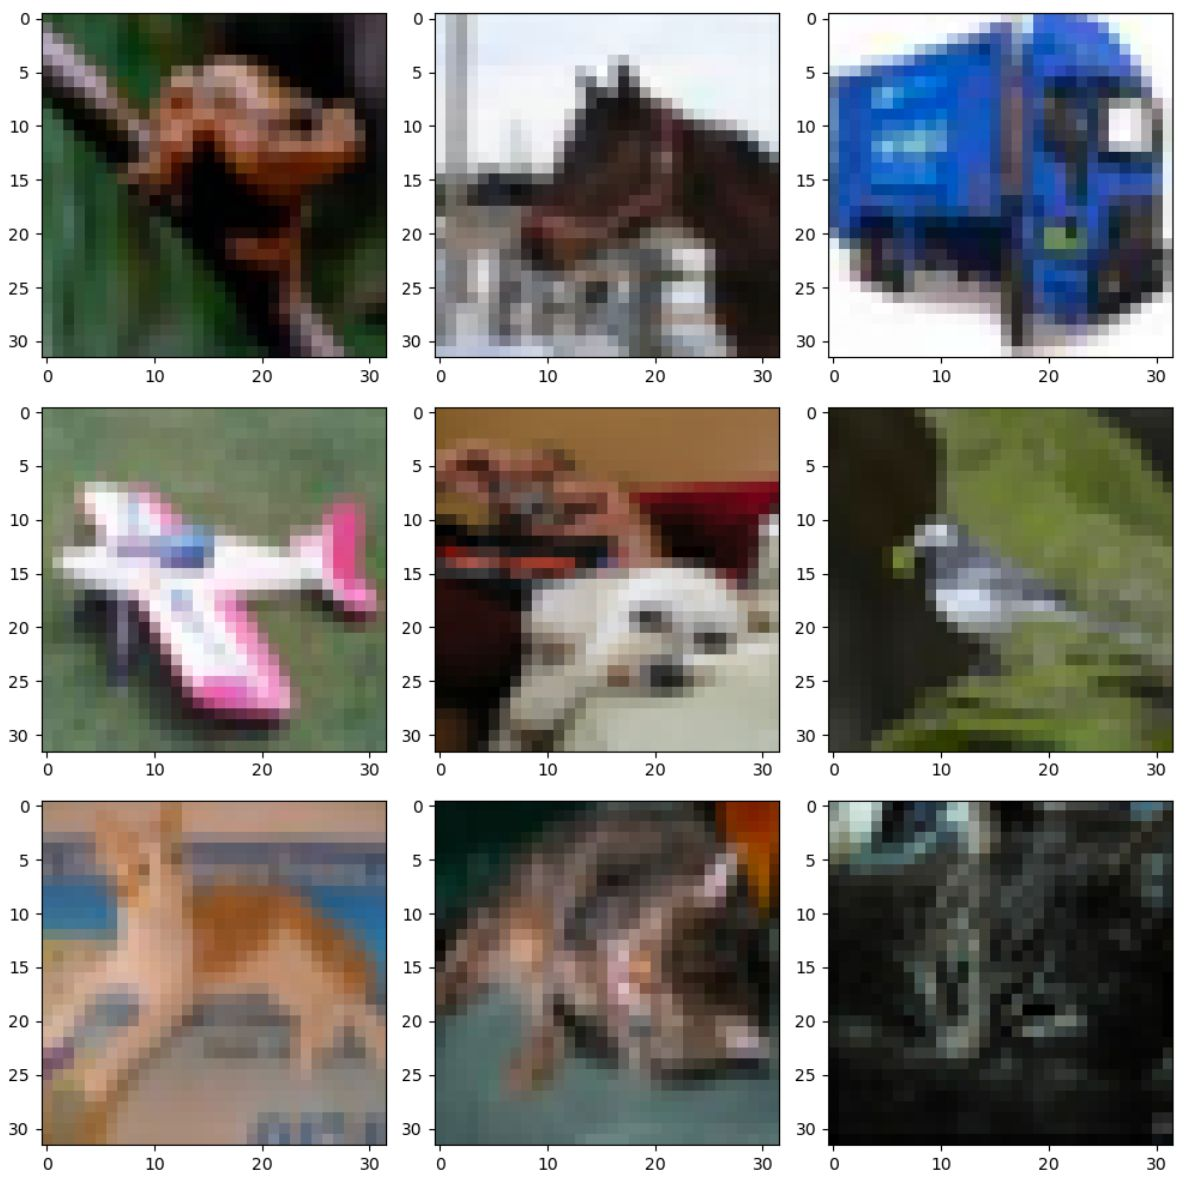
\includegraphics[width=0.8\textwidth]{Images/CIFAR}
		\caption{First nine images from the CIFAR-10 dataset.} \label{fig:cnnFirstNineCifar10}
	\end{figure}
	
	\subsection{CNN Model Definition}
	
	A Convolutional Neural Network (CNN) model is defined in Listing \ref{code:cnnDefinition} using Keras with convolutional layers, max pooling, dropout for regularization, and dense layers.
	
	\begin{code}[h!]
		\lstinputlisting[language=Python, numbers=none, linerange={199-207}]{CNN/CNN.py}    
		
		\caption{Defining a Convolutional Neural Network (CNN) model using Keras}
		\label{code:cnnDefinition}
	\end{code}
	
	\subsection{Compile the Model}
	
	In Listing \ref{code:cnnCompileModel} the model is compiled with the specified loss function, optimizer, and evaluation metric.
	
	\begin{code}[h!]
		\lstinputlisting[language=Python, numbers=none, linerange={223-223}]{CNN/CNN.py}    
		
		\caption{Compiling the CNN model with specified loss function, optimizer, and metric}
		\label{code:cnnCompileModel}
	\end{code}
	
	\subsection{Train the Model with Augmented Data}
	
	In Listing \ref{code:cnnTrainAugmented} the model is trained using the augmented data generators. This involves calling the \PYTHON{fit\_generator} function instead of \PYTHON{fit} and providing the data generators for training and validation sets.
	
	\begin{code}[h!]
		\lstinputlisting[language=Python, numbers=none, linerange={238-247}]{CNN/CNN.py}    
		
		\caption{Training the CNN model with augmented data using data generators}
		\label{code:cnnTrainAugmented}
	\end{code}
	
	\subsection{Plotting the Loss and Accuracy Curves}
	
	In Listing \ref{code:cnnLossAccuracyPlot} the accuracy and loss curves are plotted.  The somewhat unconventional scenario of validation loss being below training loss and validation accuracy exceeding training accuracy could be influenced by effective data augmentation, contributing to the model's robustness. These trends collectively suggest that the model is not overfitting the training data and is likely to generalize well to unseen data, highlighting successful training and potential for further improvement.
	
	\begin{code}[H]
		\lstinputlisting[language=Python, numbers=none, linerange={263-284}]{CNN/CNN.py}    
		
		\caption{Plotting the loss and accuracy curves}
		\label{code:cnnLossAccuracyPlot}
	\end{code}
	\subsection{Further Reading}	
	Utilizing Convolutional Neural Networks (CNNs) for license plate detection with YOLOv5 encompasses a variety of resources tailored to this specific application. While there may not be a single comprehensive source covering all aspects, a combination of research papers, tutorials, code repositories, and community discussions can provide valuable insights.
	Start with exploring research papers that focus on object detection with CNNs, particularly those that discuss YOLOv5 or related models in the context of license plate detection. Additionally, tutorials and blog posts that demonstrate the implementation of YOLOv5 for custom object detection tasks, with a focus on license plates, offer practical guidance. These resources often provide step-by-step instructions, code snippets, and tips for optimizing model performance.\newline
	For a hands-on approach, delve into code repositories on platforms like GitHub that provide pre-trained models, datasets, and training scripts specifically tailored for license plate detection using YOLOv5. Engaging with the developer community through forums, such as GitHub discussions or specialized forums for computer vision and deep learning, allows for collaboration, troubleshooting, and sharing of best practices.\newline
	Moreover, considering the interdisciplinary nature of license plate detection  involving aspects of computer vision, machine learning, and domain-specific knowledge – expanding your knowledge beyond CNNs and YOLOv5 to include topics such as image preprocessing, dataset curation, and post-processing techniques can further enhance your understanding and proficiency in this area. By leveraging these diverse resources, you can develop a comprehensive understanding of using CNNs and YOLOv5 for license plate detection, enabling you to tackle real-world applications effectively.

